
\part{\textbf{Part III - The Solutions to Diabetes}}

\newpage
~\phantom{a}
\thispagestyle{empty}
\newpage

\chapter{Diet for Diabetes, Medical Nutrition Therapy (MNT)}\label{chap22}

Diabetes is as ancient as mankind itself, and so are the basic principles of managing this disease, which revolve around three major concepts—food, exercise, and drugs. This is known as the triad of diabetes\break management. This triad is as ancient as the Egyptian pyramids, and in fact, Egyptian scriptures recovered from 1552 BC recommend a diet of wheat, berries, honey and grapes to manage diabetes!

Foremost in the triad of diabetes management is food because food is the source of glucose in the blood. Second in the triad is exercise,\break because exercise burns this glucose and hence prevents hyperglycemia. Third in the triad is medication used to control blood glucose levels.

In this chapter, we will focus on managing nutrition in diabetes, and how we can outsmart diabetes by eating smart!

Good food is one of the simplest, yet greatest joys of our lives.\break Contrary to popular belief, diabetes is a not a call to take up “sanyasa”, and relinquish the pleasures of good food. In fact, the current concept of “all food can fit” encourages people with diabetes to eat a wide\break variety of foods, as long as they are well balanced. This was not always the case though and diabetics in previous centuries were subjected to very harsh diets.

\noindent{\textbf{History of diabetic diets}}

It is very interesting to look at the history of diets recommended for diabetes. It reflects the evolution in the understanding of diabetes itself. From the ancient times to almost through 1776 when Dobson recommended a diet of large quantities of sugar and honey to\break manage diabetes, efforts were made to replace the sugar lost through urine!

In 1891, Saundby realized that feeding diabetics more sugar was not a good idea, and instead recommended a diet mostly composed of meat, vegetables and gluten bread, and encouraged his patients to eat more fat!

Between 1915 and 1921, Dr Frederick M. Allen who worked with Dr. Elliott P. Joslin (of Joslin Clinic fame), recommended a drastically restricted diet of 1000 calories per day for adults (who normally need 2000–3000 calories per day) and 400 calories per day for children, in a desperate attempt to keep blood sugars under control. While this diet did manage to control blood sugar, the severe calorie restriction\break resulted in patients dying from starvation, and hence critics labeled this diet ‘starvation diet’. Dr. Allen’s most famous patient was the 11–year old daughter of the Governor of New York. In this period, children with diabetes rarely survived more than a few months after being dia\-gnosed with diabetes. Dr. Allen placed this 11–year old girl on a daily diet of 500 calories. The girl's weight dropped from 75 lbs to 45 lbs. Unable to watch her daughter wither away in front of her eyes, her mother reached out to Frederick Banting who had discovered insulin in 1921. Banting treated the girl with insulin and gave a more humane diet. The results were miraculous. The girl got better, graduated from college, married, had 3 children, and lived to the age of 73!$^{\text{\cite{chap22–key01}}}$$^,$$^{\text{\cite{chap22–key02}}}$

Dr. Allen’s “starvation diet” found few backers as other physicians realized that most of the sugar in the blood came from carbohydrates, and hence chose to restrict carbohydrates. But in order to provide\break sufficient calories, they replaced carbohydrates with fat. For example, at the London Hospital in 1931 diabetic patients were on a diet that was 68\% fat, 17\% protein and 15\% carbohydrate.

But soon physicians such as Dr. Joslin grew concerned about the increased heart disease in diabetic patients who were being fed such a high fat diet. This resulted in another shift in diabetic diet. The era between 1950–1970 witnessed a gradual increase in carbohydrate\break proportions in the diabetic diet, with decrease in the proportion of fat.

By 1970, there was growing focus on the type of carbohydrate\break consumed, and the concept of glycemic index\index{Glycemic index} gained popularity. It was seen that some foods not only slowed down the spike in blood\break glucose after eating, but also resulted in a smaller spike in blood\break glucose levels. These were termed low glycemic index foods and\break included food items like whole grain cereals, whole fruits, etc.

The 1970s also witnessed a growing interest in dietary fiber, which was found to result in lower blood sugar levels.

In 1979, the American Diabetic Association recommended that\break carbohydrates should not be unduly restricted from the diabetic diet, as long as they came from low glycemic index sources!

Thus the diabetic diet has come a full circle, starting from high\break carbohydrate in ancient times, to low carbohydrate diet in the 18–19th century, to a carbohydrate diet without undue restrictions in the 20th century.

\noindent\textbf{Diabetic diet in the 21st century}

It may sound strange, but there is no particular special “diet”\break for diabetics in this day and age. Instead there are goals that need\break to be met with regard to blood sugar levels. To achieve these goals, dietary choices are adjusted. However, a “one–size–fits–all” approach is avoided when making these dietary adjustments. Instead, there is a persona\-lized approach, with individualized recommendations based on a person’s age, weight, sex, blood glucose levels, presence or\break absence of other medical conditions such as hypertension, heart\break disease, high cholesterol, kidney disease, etc. This personalized\break approach should also take into account the person’s ethnicity, cultural background, regional eating habits, etc. This strategy is termed\break “Medical Nutrition Therapy (MNT)”\index{Medical Nutrition Therapy (MNT)}.

\clearpage

\noindent The goals of MNT are as follows:

\vspace{-\topsep}
\begin{enumerate}[•]
\itemsep=0pt
\item Optimizing control of blood sugar levels to prevent complications\break of hyperglycemia.
\item Achieving good lipid levels to prevent the risk of cardiovascular\break disease and other vascular complications (stroke, nephropathy etc).
\item Maintaining blood pressure below 130/80 mm Hg.
\item Maintaining ideal body weight.
\end{enumerate}
\vspace{-\topsep}

To help individuals achieve these goals, MNT makes realistic\break recommendations about every single component of our daily diet. In order to appreciate this, we need to take a close look at our diet.

Let us now get to know about what our everyday food is composed of.

There are 3 main components to our daily diet, and they are also called macronutrients. They include:

\vspace{-\topsep}
\begin{enumerate}
\itemsep=0pt
\item Carbohydrates
\item Proteins
\item Fats.
\end{enumerate}
\vspace{-\topsep}

The recommended proportion of these macronutrients in our daily diet should be as follows:

\begin{figure}[h]
\centering
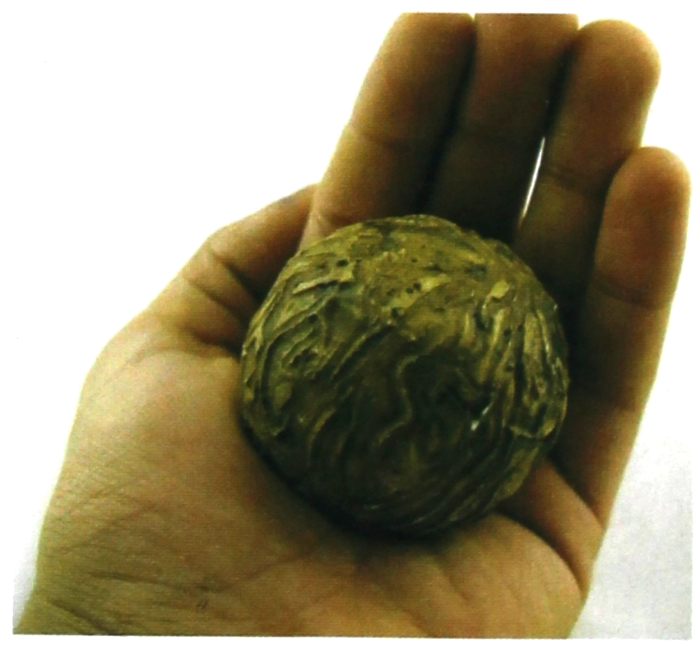
\includegraphics[scale=2]{images/077.jpg}
\vskip-.3cm
\end{figure}

Regardless of whether we consume carbohydrate, protein or fat, all foods are ultimately converted into energy within our body. This energy is measured in terms of calories. Fats provide more energy than carbohydrates or proteins.

\begin{center}
\begin{tabular}{|c|c|}
\hline
\textbf{Macronutrient} & \textbf{Energy per gm}\\
\hline
Carbohydrate & 4 calories\\
\hline
Protein & 4 calories\\
\hline
Fat & 9 calories\\
\hline
\end{tabular}
\end{center}

The body utilizes exactly as much energy as it needs, and the rest goes into storage, mostly as fat. The recommended/required daily\break caloric intake should be as follows:

\begin{center}
\begin{tabular}{|c|c|c|}
\hline
 & \textbf{Sedentary} & \textbf{Active}\\
\hline
Female (55 Kg) & 1900 kcal/day & 2230 kcal/day\\
\hline
Male (60 Kg) & 2320 kcal/day & 2730 kcal/day\\
\hline
\end{tabular}
\end{center}

With this background, let us now address each individual macro\-nutrient.

\noindent\textbf{Carbohydrate}

Carbohydrates are the primary source of calories worldwide, and especially so in the Indian diet. It is the predominant nutrient in foods we consume everyday like rice, ragi, roti, idli, dosa, bread, biscuit, and even vegetables and fruit. In fact, all foods except meat, fish and eggs, contain carbohydrate.

Carbohydrates are not only the primary source of calories, but\break foods that contain carbohydrates are also the chief source of fiber and micronutrients as well. Ideally carbohydrate should provide 45–60\% of our total calorie intake daily.

All carbohydrates are broken down to form glucose in our bodies. Hence, carbohydrates are the chief source of sugar in our blood, and sometimes carbohydrates are also called “sugars”. But this does not make carbohydrate a diabetic’s adversary. It can be a friend, as long as we choose the right carbohydrates to eat. What do we mean by “right” carbohydrate. How many types of carbohydrates are there?

\begin{center}
\begin{tabular}{|l|l|l|}
\hline
\multicolumn{1}{|c}{\textbf{Type of Carbo-}} & \multicolumn{1}{|c}{\multirow{2}{4cm}{\textbf{Naturally found in diet}}} & \multicolumn{1}{|c|}{\multirow{2}{2.3cm}{\textbf{Added to diet}}}\\
\multicolumn{1}{|c|}{\textbf{hydrate}} & &\\
\hline
\textbf{Simple} & • Glucose & Ice cream, cake\\
\hline
 & • Fructose (fruit juices, & sweetened juices,\\
  & \,\, honey) & cookies or biscuits,\\
  & • Sucrose (cane sugar & candy, etc\\
  & \,\, juice) & \\
\hline
\textbf{Complex} & All grains, vegetables, &\\
 & fruits, whole wheat bread &\\
\hline
\end{tabular}
\end{center}

\noindent\textbf{The problem with simple sugars}

Simple sugars are called so because they usually have a simple\break biochemical structure, usually with 1 or 2 rings as shown below.

\begin{wrapfigure}{r}{5.5cm}
\vskip-.4cm
\centering
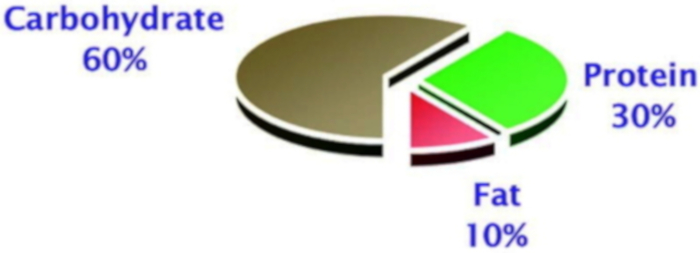
\includegraphics[scale=1.2]{images/078.jpg}
\vskip-.4cm
\end{wrapfigure}

These sugars are very easy to digest. In fact, most of these sugars are digested by\break enzymes found in the saliva\break (called amylase). The result is that they are rapidly absorbed in to the blood stream and cause a spike in the blood glucose level. Such a rapid spike stresses the pancreas, which has to rapidly pump insulin into the blood stream.

The second problem with simple sugars is that they have a high glycemic index. This means that they produce a higher blood glucose level per gram compared to substances that have a low glycemic index. In fact, the glycemic index of glucose is 100!

\begin{figure}[h]
\centering
\textbf{\textit{Blood sugar level after eating}}\\
\vskip 6pt
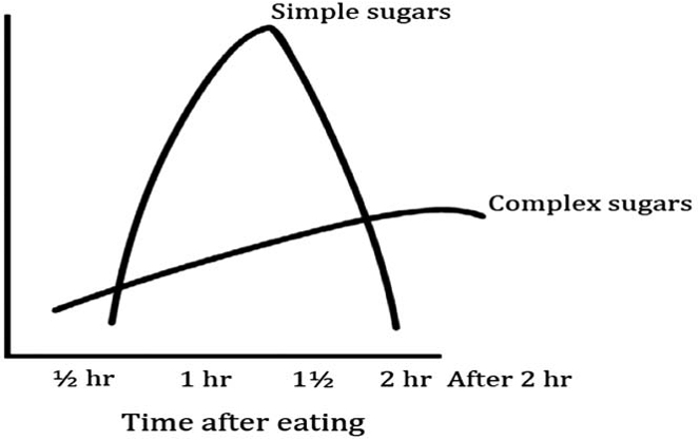
\includegraphics[scale=2.2]{images/079.jpg}
\vskip-.5cm
\end{figure}

Thus, simple sugars not only cause a rapid rise in blood sugar\break levels, but also cause a higher peak blood sugar level. This results in increased stress on the pancreas, and excess glucose in blood, which will eventually transform into advanced glycation end–products (ACE), which harm our organs.

\noindent\textbf{The benefit of complex carbohydrates}

Complex sugars have a multi–ringed structure as shown below.\break Because of this complex structure, it takes longer for the digestive\break enzymes to break this structure down to produce glucose. The result is a slow rise in blood sugar level that does not overwhelm the pancreas.

\begin{wrapfigure}{r}{6.5cm}
\vskip-.4cm
\centering
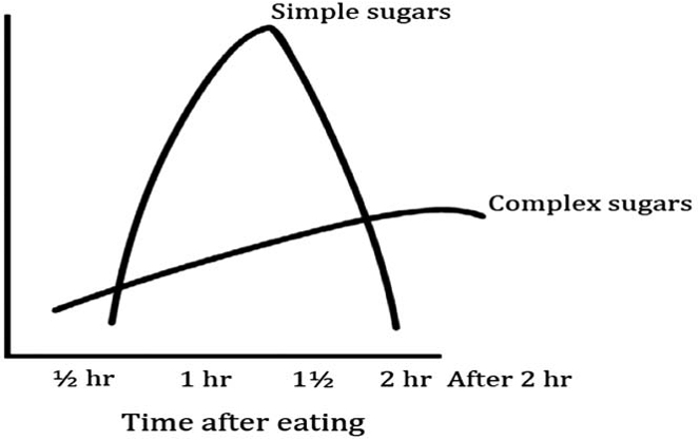
\includegraphics[scale=1.4]{images/080.jpg}
\vskip-.2cm
\end{wrapfigure}

In addition, the entire complex carbohydrate\break cannot be broken down and the body cannot\break extract all the available sugar in it. Hence there is a smaller blood glucose peak after consuming a complex sugar. By definition, this makes it a low glycemic index food.

Additionally, complex carbohydrates have a naturally occurring fiber in them. Fiber further delays glucose release from these foods. Fiber has many other health benefits, and they are detailed later in the chapter.

\clearpage
Finally, complex sugars have several micronutrients in them. For example whole grains (unpolished grains) are a treasure trove of\break vitamins and minerals. They are rich in anti-oxidants as well.

As a society we have an incessant obsession with all things fair\break and white. Unfortunately, we have taken this obsession too far by\break polishing our rice till they are ‘pearl white’ as well. Have you seen any naturally found food in this world that is pearl white? The truth is that the darker the grain or vegetable, the more nutritious it is.

\begin{center}
\begin{tabular}{|l|l|}
\hline
\textbf{The current problem} & \multicolumn{1}{c|}{\multirow{2}{5cm}{\textbf{Solutions to these problems}}}\\
\multicolumn{1}{|c|}{\textbf{with carbohydrates}} &\\
\hline
Excess added sugar & Avoid carbonated beverages\\
 & such as Coke, Pepsi, etc.\\
 & Avoid high calorie snacks such\\
 & as cookies, candy, chocolate etc.\\
 & Instead eat fruits and vegetables,\\
 & and drink more water\\
\hline
Emphasis on using & Avoid using polished rice.\\
refined grains & Use ragi and whole wheat\\
 & flour Avoid \textit{maida}\\
\hline
Inadequate fiber & Incorporate more whole grains in diet.\\
 & Consume more vegetables and fruits\\
\hline
\end{tabular}
\end{center}

\noindent\textbf{Protein}

Protein is in every cell of our body, and is in fact the whole and soul of human cells. They not only function as enzymes catalyzing\break millions of biochemical reactions inside the cells, but also form the cell\break membranes to maintain the integrity of the cells. They also function as messengers between cells. They are essential for us to maintain our muscle mass. They are also the second most important source of calories, next only to carbohydrates. About 30\% of daily calorie intake should come from proteins.

\noindent Protein is found in many sources, both plant and animal based.

\vspace{-\topsep}
\begin{enumerate}[\ding{118}]
\itemsep=0pt
\item Plant sources include beans, lentils (dals), peas, nuts, seeds, etc.
\item Animal sources include meat (red meat such as lamb, goat, sheep, beef, pork), chicken, fish and other seafood, eggs, milk and milk products. It is preferable to avoid red meat sources of protein, as they are more likely to have excess cholesterol and are unhealthy in general.
\end{enumerate}
\vspace{-\topsep}

Daily requirement of protein varies by age, body weight, daily\break activity level, and condition of kidneys. But to simplify matters, daily intake of 0.8 mg/kg for adults should be adequate. In patients with nephropathy (kidney disease), it is reasonable to reduce protein intake to about 0.6 mg/kg/day to reduce the workload on the kidneys, since all protein has to be excreted through the kidneys.

Proteins have special advantages when it comes to diabetes. They provide a sense of satiety or fullness after eating them. Also, it tends to suppress hunger. As a result, a protein–rich meal can prevent needless snacking after meals, which causes blood sugars to go out of control. Furthermore, proteins do not cause a spike in blood glucose levels after eating them, as opposed to carbohydrates. Hence though they are a source of calories, they do not disrupt blood sugar control.

\noindent\textbf{Fats}

As mentioned in the chapter on lipids, hyperlipidemia and heart disease is 2–4 times higher in patients with type 2 diabetes when\break compared to the general population, and this a direct result of eating too much fatty food and leading a sedentary life.

But fat need not be our enemy. As a matter of fact, fat is an\break essential component of our food. It supplies essential fatty acids, and also helps us absorb certain vitamins, namely vitamins A, D, E and K. Obviously, dietary fat is associated with both health benefits and\break significant risks. The mantra when it comes to dietary fat is not only how much fat to eat, but also what type of fat to eat. So what are the types of fat available in our diet?

\clearpage

{
\addtolength{\tabcolsep}{-6pt}
\begin{longtable}{|l|l|l|l|}
\hline
\multicolumn{1}{|c|}{\multirow{2}{2.3cm}{\textbf{\,\,\,Type of fat}}} & \multicolumn{1}{c|}{\multirow{2}{3.1cm}{\textbf{\,\,\,Dietary Sources}}} & \textbf{What does it do} & \multicolumn{1}{c|}{\textbf{What does this}}\\
 &  & \multicolumn{1}{c}{\textbf{in our body?}} & \multicolumn{1}{|c|}{\textbf{mean for you?}}\\
\hline
\textbf{\textit{Saturated fat\index{Saturated fat}}} &  &  & \\
(Solid at room & Animal source & Increases LDL & \textless 7\% of total daily\\
temperature) & fats such as butter, &  & calorie intake\\
 & cream, ghee and &  & should come from\\
 & cheese. Plant &  & saturated fats. Eat\\
 & source fats such as &  & as little of this as\\
 & coconut oil, palm &  & possible\\
 & kernel oil &  & \\
\hline
\textbf{\textit{Trans fat\index{Transfat}}} &  &  & \\
(Solid at room & Hydrogenated oils & Increases LDL & Avoid this if you\\
temperature) & (Dalda, Vanaspathi, & Decreases HDL & can, if not eat the\\
 & margarine, salad &  & least possible\\
 & dressings, baked &  & amount\\
 & foods, etc) &  & \\
\hline
\textbf{\textit{Monounsatu-}} &  &  & \\
\textbf{\textit{rated fats\index{Monounsaturated fats}}} &  &  & \\
(Liquid at & Olive oil, mustard & Decreases LDL & 10-20\% of daily\\
room & oil,canola oil, nuts, & Increases HDL & calorie intake\\
temperature) & avocado &  & should be from\\
 &  &  & these type of fats\\
\hline
\textbf{\textit{Polyunsatu-}} &  &  & \\
\textbf{\textit{rated fats}} &  &  & \\
(Liquid at & Sunflower oil, & Decreases LDL & \textless 10\% of daily\\
room & groundnut & Decreases & calorie intake\\
temperature) & (peanut) oil, & Cholesterol & should be from\\
 & safflower oil, &  & these type of\\
 & corn oil, flaxseed &  & fats\\
 & oil, soya bean oil &  & \\
\hline
\end{longtable}
}\relax

\begin{quote}
\textit{\textbf{Note:} Remember that LDL is the bad cholesterol that you do not want, and HDL is the good cholesterol that you do want in your blood.}
\end{quote}

Thus, in general plant–based fats are better than animal source fats. Natural fat (found in seeds and nuts) is better than added fat (which is unfortunately a more common source of fat in our diets).

Another point to keep in mind about fats is that our daily\break cholesterol intake should be less than 300 mg. And in patients with cardiovascular disease risk, it should be less than 200 mg per day. You may be surprised to know that our body synthesizes all the cholesterol that we need on its own, and it is not essential for us to get cholesterol in our diet!

Another popular fad in our diets today is the so–called “fat–free” products. Many of these snacks contain “fat replacers”, which help maintain taste. These fat replacers are usually made out of carbohydrates and some protein. So even though we tend to feel good about eating these fat–free snacks, due to the carbohydrate present in them, the blood sugar levels can increase on eating these types of foods.

Fiber can be our friend when it comes to cholesterol and lipids, because it helps to decrease cholesterol, LDL and triglycerides, without adversely affecting HDL (the good cholesterol).

\noindent\textbf{Dietary fiber}

Fiber comes purely from plant sources. It is also called “roughage”. There are two kinds of fiber:

\vspace{-\topsep}
\begin{enumerate}
\itemsep=0pt
\item Soluble fiber– this will dissolve in water; when dissolved in\break water, it forms a viscous (thick) gel. This gel slows down the movement of food through the digestive system. Also, this gel coats the inner walls of the intestines and interferes with the\break activity of digestive enzymes, and hence delays absorption\break of glucose into the blood. Sources of soluble fiber include the following:
\vspace{-\topsep}
\begin{enumerate}[a)]
\itemsep=0pt
\item Legumes – peas, soya bean, other beans
\item Grains– oats, rye, barley
\item Fruits
\item Vegetables
\item Flax seeds
\item Nuts
\end{enumerate}
\vspace{-\topsep}
\item Insoluble fiber– this type of fiber does not dissolve in water.\break They absorb water as they move through the digestive tract,\break and hence make the stools soft and bulky, and thereby\break avoiding constipation. They also tend to accelerate movement of food through the digestive tract. Sources of insoluble fiber include:
\vspace{-\topsep}
\begin{enumerate}[a)]
\itemsep=0pt
\item Legumes– beans and peas
\item Grains– wheat, corn
\item Some fruits such as unripe bananas, and skins of fruits
\item Vegetables and their skins
\item Nuts and seeds
\end{enumerate}
\end{enumerate}
\vspace{-\topsep}

\noindent The many benefits of dietary fiber are listed below:

\vspace{-\topsep}
\begin{enumerate}[•]
\itemsep=0pt
\item Fiber increases the volume of food without adding any calories. The increased volume of food gives a sense of being full, and hence\break decreases total food intake.
\item Soluble fiber forms a viscous gel that slows down the movement\break of food through the digestive system. The gel also interferes with\break digestive enzyme activity. The result is a slow and incomplete\break absorption of dietary glucose into the blood. This prevents a sudden and significant blood sugar spike after eating.
\item By adding bulk and by slowing down movement of food, fiber\break suppresses hunger.
\item Soluble fiber binds to the bile acids present in bile juice. This\break decreases the amount of fat absorbable from diet.
\item Fiber decreases glucagon release, and hence indirectly helps insulin action.
\item Insoluble fiber makes the stool bulky and soft and prevents consti\-pation.
\end{enumerate}
\vspace{-\topsep}

Many of these benefits were demonstrated scientifically by a study done at the University of Texas Southwestern Medical Center in Dallas, Texas. In this study, patients with type 2 diabetes were given food that contained 24 gm of fiber per day for 6 weeks. These same patients were later given a diet that contained 50 gm of fiber daily for 6 weeks. It was found that when patients consumed more fiber (50 gm per day versus 24 gm per day), they had a 6.7\% lower fasting blood glucose, 10.2\% lower triglyceride level, 6.3\% lower LDL (bad cholesterol) level, and 12.5\% lower VLDL (bad cholesterol) level. This study showed that in just 6 weeks dietary fiber can improve both blood sugar control and cholesterol levels.$^{\text{\cite{chap22–key03}}}$

\noindent\textbf{Practical tips when consuming dietary fiber}

\vspace{-\topsep}
\begin{enumerate}[•]
\itemsep=0pt
\item Drink plenty of water with fiber. This will prevent excess gas\break formation and also, it helps fiber form a gel inside the intestines.
\item Increase fiber content in the diet slowly over weeks. Suddenly\break starting to eat 50 gram of fiber per day can cause a lot of abdominal gas.
\item Avoid juices and instead eat whole fruits. Similarly avoid cooking vegetable excessively, since this not only destroys the nutrients, but also breaks down the fiber in these vegetables.
\end{enumerate}
\vspace{-\topsep}

\noindent\textbf{Salt}

The role of salt in our lives is captured very well in this ancient proverb, \textit{“Three things are good in small doses, and bad in big doses– yeast, salt and hesitation”}.

Salt is essential not only to keep our taste buds happy, but also\break to keep us alive. It is salt that maintains the fluid balance within our bodies and our cells, because without it our cells would shrink and die. It is salt (sodium and chloride ions) that is key to our heartbeat, and for contraction and relaxation of other muscles in our body. Salt is also\break essential for our nerves to communicate with each other, and with other cells and organs in our body.

But it is said that “good things come in small packages”, and so is true of salt. We only need about 3 grams of salt daily. You will be surprised to know that 3 grams per day is more than enough to keep our blood as salty as seawater! The daily requirement of salt is the same in both diabetics and non–diabetics.

Salt restriction to less than 2.4 grams per day is advised for patients with hypertension, kidney disease (nephropathy), and heart failure. This is because salt tends to absorb water and thus retains more fluid in the human body. This excess fluid volume worsens hypertension, and heart failure. In case of nephropathy, the damaged kidneys are unable to get rid of the excess (or even normal) amounts of water content in the body.

\noindent\textbf{Artificial sweeteners}

These are attractive alternatives to sugar for diabetics since they are supposed to have practically no calories, while still imparting\break sweetness to foods. Thanks to these sweeteners, bitter sugarless teas or coffee is a thing of the past for diabetics. These sweeteners can also help diabetics control their weight. They are several hundred times sweeter than sugar, and hence need to be used in much smaller quanti\-ties than sugar. Some of them can even be used to cook foods, since they are heat–stable. Some of the commonly used artificial sweete\-ners are listed in the following table.

{
\addtolength{\tabcolsep}{-5pt}
\begin{longtable}{|c|c|c|c|}
\hline
\multicolumn{1}{|c|}{\multirow{2}{1.6cm}{\textbf{Artificial}}} & \textbf{How many} &  & \textbf{Can you}\\
\multicolumn{1}{|c|}{\multirow{2}{1.6cm}{\textbf{Sweetener}}} & \textbf{times sweeter} & \textbf{Brand names} & \textbf{cook with}\\
 & \textbf{than sugar?} &  & \textbf{it?}\\
\hline
\textbf{Acesulfame K} & 200 times & Sunette, Sweet & Yes\\
 &  & One (in USA) & \\
\hline
\textbf{Aspartame} & 160-220 times & Equal, Sugarfree & Not reco-\\
 &  & Nutrasweet (USA) & mmended\\
\hline
\textbf{Saccharin} & 200-700 times & Sweet’N Low (USA) & Yes\\
\hline
\textbf{Sucralose} & 600 times & Splenda, Zero & Yes\\
 &  & Calorie & \\
\hline
\end{longtable}
}\relax

\noindent\textbf{Vitamins and minerals}

These are also called micronutrients, since they are required in very small quantities on a daily basis. They comprise a large group and include iron, copper, magnesium, vitamins, etc. A balanced diet\break consisting of vegetables, fruits, nuts, seeds, dairy products, eggs, fish, etc is the best source of these micronutrients. However, in some\break situations there is a need to monitor for deficiency of some of these micronutrients and to replace them. Such situations include:

\vspace{-\topsep}
\begin{enumerate}[•]
\itemsep=0pt
\item Diabetics with poor blood sugar control may lose an excess of some of the micronutrients due to excessive urination.
\item Diabetics who are hypertensive and are treated with diuretic\break medications (water pills) have increased urination and may lose\break micronutrients.
\item Some medications can inhibit absorption of minerals and vitamins. For example, metformin can inhibit absorption of vitamin B12.
\item Strict vegetarians may be at risk to certain micronutrient defici\-encies such as vitamin B12.
\item Diabetic women who are pregnant have an increased nutritional\break requirement.
\item Women who have excess blood loss during menstruation are at the risk of anemia, and need iron supplementation.
\item Older women are at the risk of osteoporosis\index{Osteoporosis} (weak bones) due to\break calcium deficiency and vitamin D deficiency.
\item Elderly individuals have a low appetite and hence do not consume enough nutritious food.
\item Individuals who are trying to lose weight and are “dieting”.
\end{enumerate}

\noindent\textbf{A spicy way to control blood sugar: the role of spices in a diabetic’s diet}

It is said that familiarity breeds contempt. Spices are so ingrained in our diets that we do not pause to think about the many health\break benefits they bestow upon us. But this fact was not lost on our\break ancestors who invented and practised the ancient Indian systems of medicine, namely Ayurveda, Siddha, Unani and Yoga. It is now that the entire world is rediscovering the magic of Indian spices. The\break following table lists the various scientifically proven health benefits of the commonly used spices in our kitchens everyday.

\vskip 12pt
\begin{longtable}{|l|l|}
\hline
\multicolumn{1}{|c|}{\textbf{Spice}} & \multicolumn{1}{c|}{\textbf{Health Benefit}$^{\text{\cite{chap22–key04}}}$$^,$$^{\text{\cite{chap22–key05}}}$$^,$$^{\text{\cite{chap22–key06}}}$}\\
\hline
Cardamom (elaichi) & Decreases blood pressure\\
\hline
Cinnamon \textit{(dalchinni)} & Decreases insulin resistance\\
\hline
Coriander \textit{(dhania)} & Decreases blood glucose, increases\\
 & insulin release\\
\hline
Cumin \textit{(jeera)} & Decreases blood glucose and\\
 & cholesterol\\
\hline
Curry leaves \textit{(kadi patha)} & Decreases blood glucose and\\
 & cholesterol\\
\hline
Fenugreek \textit{(methi)} & Decreases blood glucose, insulin level,\\
 & cholesterol \& triglyceride\\
\hline
Garlic & Lowers blood glucose, blood pressure\\
 & \& cholesterol\\
\hline
Ginger & Lowers blood pressure\\
\hline
Mustard seeds/black & Lowers blood glucose \& cholesterol\\
\hline
Mustard (sarson/rai) &\\
Pepper (kali mirch) & Lowers blood glucose \& cholesterol\\
\hline
Nutmeg \textit{(jaiphal)} & Lowers blood glucose \& cholesterol\\
\hline
\end{longtable}

\noindent\textbf{Summary}

The following table summarizes what was discussed throughout this chapter and can serve as a guide for diabetics to make smart choices with food.

\clearpage

{
\small\addtolength{\tabcolsep}{-5pt}
\begin{longtable}{|l|l|l|l|}
\hline
\multicolumn{1}{|c}{\textbf{Food}} & \multicolumn{1}{|c}{\textbf{Can Consume in}} & \multicolumn{1}{|c}{\textbf{Consume in}} & \multicolumn{1}{|c|}{\textbf{Avoid or Consume}}\\
\multicolumn{1}{|c}{\textbf{categories}} & \multicolumn{1}{|c}{\textbf{large quantities}} & \multicolumn{1}{|c}{\textbf{moderation}} & \multicolumn{1}{|c|}{\textbf{very sparingly}}\\
\hline
\textbf{Carbo-} & Wheat bread, & White bread, & Cookies, biscuits,\\
\textbf{hydrates} & brown rice, whole & white (polished) & cake, jam, maida\\
 & grains, wheat, ragi, & rice & \\
 & corn, bajra &  & \\
\hline
\textbf{Protein} & Dal, lentils, beans & Chicken, fish, & Red meat—goat,\\
 &  & egg white, & sheep, beef,\\
 &  & whole milk & pork; egg yolk\\
\hline
\textbf{Fats} & Buttermilk & Olive oil, & Butter, ghee,\\
 & without cream & mustard oil, & cheese, dalda,\\
 &  & canola oil, & coconut oil,\\
 &  & sunflower oil, & palm oil\\
 &  & groundnut oil, & \\
 &  & corn oil, & \\
 &  & flaxseed oil, & \\
 &  & soya bean oil, & \\
 &  & avocado, nuts & \\
\hline
\textbf{Vegetables} & All except those & Carrot, beetroot, & Potato\\
 & listed in table & peas & \\
\hline
\textbf{Fruits} &  & Apples, oranges, & Chiku (Sapota),\\
 &  & papaya, musk & banana, mango,\\
 &  & melon & jack fruit, grapes,\\
 &  &  & \textit{sitaphal} (custard\\
 &  &  & apple), dates, fig,\\
 &  &  & raisins\\
\hline
\textbf{Fluids} & Unsweetened & Tea, coffee & Coconut water,\\
 & lime juice & with artificial & colas, sodas\\
 &  & sweetener & (“cool drinks”),\\
 &  &  & Horlicks, Boost\\
\hline
\end{longtable}
}\relax

This summary can also be presented in the form a “food pyramid”. This is a concept that is popular in the United States and many other countries. The food pyramid is composed of 6 horizontal sections\break composed of different food groups namely cereals, vegetables, fruits, pulses, milk and oil. The size of these individual food sections also shows the recommended daily intake for each of these food groups.

\begin{figure}[h]
\centering
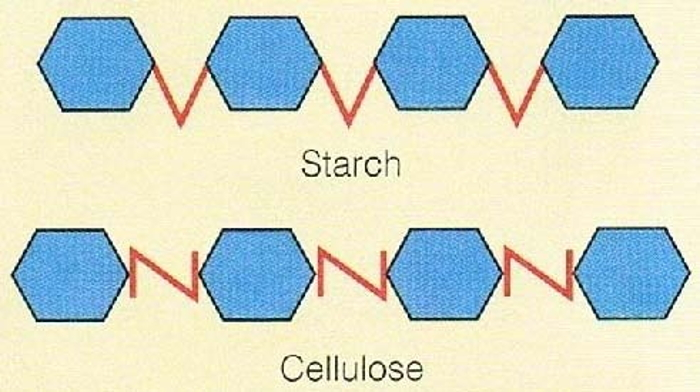
\includegraphics[scale=1.6]{images/081.jpg}\\
\textbf{\textit{Food Pyramid for Vegetarians}}
\vskip-.4cm
\end{figure}

\vspace{-\topsep}
\begin{figure}[h]
\centering
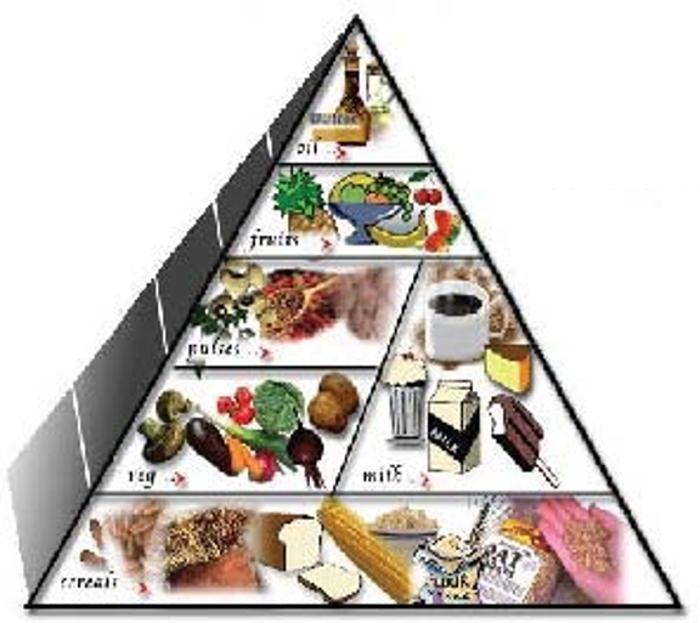
\includegraphics[scale=2.4]{images/082.jpg}\\
\textbf{\textit{Food Pyramid for Non–Vegetarians}}
\vskip-.4cm
\end{figure}

\clearpage

\begin{thebibliography}{99}
%~ \rhead[\small \em Diet for Diabetes. Medical Nutrition Therapy (MNT)]{\small\thepage}
\bibitem{chap22–key01} Joslin E: The Treatment of Diabetes Mellitus. 2nd edition. Phila\-delphia: Lea \& Febiger; 1917.
\bibitem{chap22–key02} Cox C: The Fight to Survive. New York: Kaplan; 2009.
\bibitem{chap22–key03} Chandali M, Garg A, Lutjohann D, von Bergmann K, et al. Beneficial effects of high dietary fiber intake in patients with type 2 diabetes mellitus. N Eng J Med. 2000; 342(19):1392–8.
\bibitem{chap22–key04} Iyer A, Panchal S, Poudyal H, \& Brown L. Potential health benefits of Indian spices in the symptoms of the metabolic syndrome: a review. Indian J Biochem Biophys. Dec 2009; 46: 467–81.
\bibitem{chap22–key05} Krishnaswami K. Traditional Indian spices and their health signi\-ficance. Asia Pac J Clin Nutr. 2008; 17(S1): 265–8.
\bibitem{chap22–key06} Vasanthi HR \& Parameswari RP. Indian spices for a health heart– an overview. Current cardiology reviews. 2010; 6(4): 274–9.
\end{thebibliography}

\newpage

%~ \rhead[\small \em \leftmark]{\small\thepage}
\chapter{The Role of Physical Exercise in Diabetes}\label{chap23}

\begin{quote}
\textit{All parts of the body, which have a function, if used in moderation and exercised in labour, become healthy and well developed and age more slowly. But if left unused and idle, they become liable to disease, defective in growth, and age quickly.}
\vspace{-\topsep}
\begin{flushright}
\textbf{–Hippocrates}
\end{flushright}
\end{quote}
\vspace{-\topsep}

Would it not be wonderful if there were a treatment for diabetes that was free of cost and side effects!

Yes it is true. Research has proved that physical exercise by it\-self can decrease HbA1c levels by up to 1\%. And do not underestimate the power of 1\% of HBA1c. A 1\% reduction can translate into a 21\%\break reduction in risk of stroke, heart attack and other microvascular\break complications of diabetes.$^{\text{\cite{chap23–key01}}}$

In the classical triad of diabetes management, physical exercise takes second place after food.

\noindent{\large\textbf{Regular exercise: An Important key to healthy living in diabetes}}

\noindent\textbf{How does exercise help control diabetes?}

Several biochemical changes happen in the body during exercise. As you know, the muscles are very active during exercise, and need extra energy. In the first 15 minutes of exercise, this extra energy is supplied in 2 ways:

\begin{enumerate}[•]
\itemsep=0pt
\item Increased blood flow to the muscles carries more blood glucose to the muscles
\item The glucose stores in the muscles (glycogen) are broken down to\break release more glucose.
\end{enumerate}

\vskip -.3cm

After 15 minutes of exercise, the glycogen stores in the muscles are exhausted. Now the glucose in the blood is the only source of\break energy for the muscle cells. But if the working muscles keep on\break drawing glucose from the blood, then the glucose levels will drop and the person will develop hypoglycemia. But the liver prevents this by releasing more glucose into the circulation. It does so by breaking down the glucose stores in the liver (glycogen). This process is called “glycogenolysis”\index{Glycogenolysis}.

After 30 minutes of exercise, the glycogen stores in the liver also start getting depleted. The body now turns to the fat stores for extra glucose. Fat is broken down and the byproducts are used to synthesize more glucose. This process is called “gluconeogenesis”\index{Gluconeogenesis}.

At some point in time, even this process of gluconeogenesis will get exhausted, and cannot keep up with the increased demand for glucose. As a result the glucose levels in the circulation will drop and result in hypoglycemia.

After we stop exercising, the muscles continue to take in more\break glucose to replenish their stores of glycogen that were used up\break during exercise. This process may take up to 12 to 24 hours. Hence, one of the benefits of exercise is that the blood glucose levels remain under control for up to 24 hours after exercise.

So, now you see how exercise not only controls blood sugar levels for up to 24 hours, but also can result in weight loss and decreased body fat.

\noindent\textbf{What are the benefits of exercise?}

Blood sugar remains under control for more than 24 hours after exercising. In addition, the blood sugar levels after food intake do not rise too high for more than 24 hours after exercise.$^{\text{\cite{chap23–key02}}}$$^,$$^{\text{\cite{chap23–key03}}}$

The benefit of exercise was seen long term also, i.e. beyond 24 hours. The HbA1c levels were much lower in diabetics who exercised, even if they did not lose weight.$^{\text{\cite{chap23–key04}}}$

\noindent In addition, exercise also results in:

\vspace{-\topsep}
\begin{enumerate}[•]
\itemsep=0pt
\item Decreased fasting blood sugar levels
\item Decreased insulin resistance
\item Decrease in the dose of insulin or oral medicines used to treat\break diabetes
\item Decreased blood pressure in diabetic patients with high blood\break pressure
\item Decreased body weight and abdominal obesity
\item Decreased blood cholesterol levels, with increase in HDL (the good cholesterol)
\item Increased bone strength
\end{enumerate}
\vspace{-\topsep}

Another major advantage of regular exercise is that it reduces the blood’s coagulability or clotting tendency. This is valuable because it is a blood clot in one of the narrowed, antherosclerotic coronary\break arteries, which is responsible for heart attack in general, and diabetes in particular.

\noindent Further, there are several other subjective benefits such as:

\vspace{-\topsep}
\begin{enumerate}[•]
\itemsep=0pt
\item Increased energy levels during the day
\item Better sleep at night
\item Decreased stress and feeling of anxiety or depression
\item Increased muscle strength
\item An overall feeling of wellness.
\end{enumerate}
\vspace{-\topsep}

So, in summary, several benefits accrue from a regular exercise schedule. The improvement in insulin sensitivity resulting from\break regular physical exercise is of major importance in achieving long term glycemic control. The improvement in the lipid profile as well as\break reduction of hypertension is a major effect of exercise on cardio\-va\-scular risk factors.

Exercise also helps in reducing weight, increasing stamina, and\break providing a sense of well–being, and improves overall quality of life.

\noindent\textbf{What kind of physical activity is beneficial?}

You are bound to hear several opinions about what kind of exercise you should indulge in to get the maximum benefit.

\noindent There are 2 different types of activities:

\vspace{-\topsep}
\begin{enumerate}
\itemsep=0pt
\item \textbf{Aerobic activity –} this includes walking, running, stretching, etc.
\item \textbf{Resistance activity –} such as lifting weights (or increasing\break resistance to the muscle)
\end{enumerate}
\vspace{-\topsep}

\begin{center}
\begin{tabular}{@{}cc@{}}

\includegraphics[scale=1.2]{images/083.jpg}&
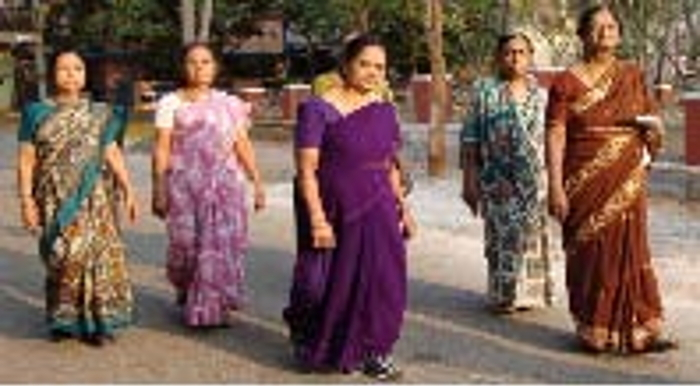
\includegraphics[scale=1.1]{images/084.jpg}\\
{\small\textbf{\textit{Stretching exercises– making the}}}&
{\small\textbf{\textit{Health–conscious Mysore ladies}}}\\
{\small\textbf{\textit{most of the many parks in Mysore}}}&
{\small\textbf{\textit{enjoying their morning walk}}}\\
\quad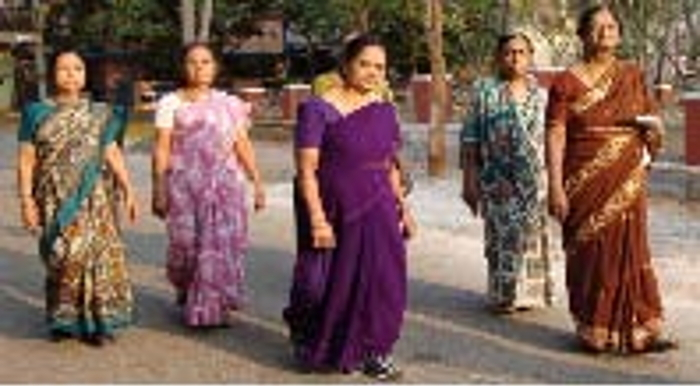
\includegraphics[scale=.9]{images/085.jpg}\\
\quad{\small\textbf{\textit{Bilateral knee joint}}}\\
\quad{\small\textbf{\textit{replacement cannot slow}}}\\
\quad{\small\textbf{\textit{down the spirit of exercise !}}}\\
\end{tabular}
\end{center}

According to clinical studies, either aerobic or resistance activity, or both combined, led to a drop in HbA1c level. please bear in mind that, whether you walk, jog, stretch, lift weights, do yoga, climb\break stairs, etc you will reap all the benefits of exercise. You should pick the activity that suits you. Someone suffering from arthritis of knee joints may find it more suitable to do resistance exercises (lifting weights, stretching, etc) than aerobic exercises such as walking or jogging.

\noindent\textbf{How much exercise is ideal?}

In general, the goal should be 30 minutes of moderate physical\break activity every day for at least 5 days of the week. But if you are like the majority of diabetics who do not indulge in any physical activity, this goal may seem like a distant dream or even a nightmare to some!

But this should not be a cause for worry.

It is recommended to start low and go slow. This gives your mind and body time to get acclimatized to exercise. A practical suggestion would be to start 10 minutes of mild activity, around 3 to 5 days of the week, and then gradually increase to 30 minutes of moderate activity for at least 5 days of the week.

In addition to duration, another goal of exercise is to attain the recommended intensity. This can be gauged by the heart rate a person achieves during exercise. A rule of thumb is that your target heart rate should be 220 minus your age. For example, if a person is aged 50 years, his target heart rate during exercise should be 220–50=170 beats per minute.

\noindent\textbf{Exercise and India}

Despite overwhelming evidence supporting the various health\break benefits of exercise, India and Indians have failed to embrace exercise as an integral part of healthy living. While the exact figures from India are unavailable, the level of inactivity among Indian immigrants in the USA, Canada and the UK is an alarming 60 to 78\%.

\clearpage

\noindent\textbf{What are the reasons behind the low levels of physical activity among Indians?}

Exercise does not have to be jogging 5 miles or\break lifting weights for half hour, etc. It can be any activity that increases heart rate for a reasonable period of time. These recommendations should be customized to the Indian public. For example physical\break activity includes playing with children or grandchildren, walking or playing with your dog, using stairs instead of the elevator, etc.

India is growing…horizontally! Obesity rates are exploding across the country. India has slowly but steadily moved away from an agri\-cul\-ture–based economy. According to a study reported in the ‘Times of India’ newspaper, in 1978 around 81\% of rural males primarily worked in agriculture. This figure has dropped to 55\% as of 2010. So how is this statistic tied to obesity? Well, agricultural work involves hard physical labor, as opposed to the service industry. Hence the society as a whole has become more sedentary, and is consuming more calories than it is burning.

\vskip 4pt
\noindent\textbf{Evaluation of diabetic patients before starting an exercise\break program and appropriate recommendations}
\vskip 4pt

The biggest secret of good health is common sense! The same is true when contemplating physical activity or exercise in diabetics.\break Diabetes creates some unique challenges with regard to physical\break activity. Exercise may aggravate several complications of diabetes if we do not take adequate precautions. The following table discusses these issues that apply to all age groups with diabetes. It also offers suggestions to overcome or prevent them.

\vskip 4pt

{
\small\addtolength{\tabcolsep}{-5pt}
\begin{longtable}{|l|l|}
\hline
\multicolumn{1}{|c|}{\textbf{Risk/Issue}} & \multicolumn{1}{|c|}{\textbf{Solution}}\\
\hline
\textbf{Risk of hypoglycemia\index{Hypoglycemia}} & \\
Usually exercise or physical activity is done & • Carry a source of easy\\
early morning, when blood sugar levels are & \,\, and quick glucose in\\
usually at their lowest due to the overnight fast. & \,\, your pocket (candy,\\
Physical activity can sometimes decrease the & \,\, chocolate, etc)\\
\hline
blood sugar levels to lower levels than usual. & • Carry a card which states\\
 & \,\, you are diabetic\\
\hline
\textbf{Risk of foot injury due to peripheral} & \\
\textbf{neuropathy\index{Peripheral neuropathy}} & \\
The preferred method of exercise is walking & • Examine your feet before\\
or jogging. Wearing ill-fitting footwear, being & \,\, and after exercise for any\\
barefoot, the sad state of our roads and public & \,\, injuries\\
parks, all increase risk of foot injury that can & • Wear the right footwear\\
result in ulcers, and eventually amputation. & • Limit weight-bearing\\
 & \,\, exercises such as lifting\\
 &\,\, weights etc\\
 & • Avoid exercise when it is\\
 & \,\, too cold or too hot\\
\hline
\textbf{Risk of retinal detachment\index{Retinal detachment} or bleeding} & \\
In patients with proliferative retinopathy, & • Regular ophthalmologic\\
certain exercises can increase risk of retinal & \,\, examination\\
detachment or bleeding & • Avoid activities that\\
 & \,\, are jarring (jogging) or\\
 & \,\, involve straining (lifting\\
 & \,\, weights)\\
 & • Walking, swimming,\\
 & \,\, water exercises are\\
 & \,\, preferable\\
\hline
\textbf{Risk of muscle or ligament strains/sprains} & \\
Starting vigorous exercise without adequate & • Perform stretching\\
warm-up. & \,\, exercises before starting\\
 & \,\, exercise\\
 & • Start walking slowly\\
 & \,\, before increasing speed\\
 & • Slow down before coming\\
 & \,\, to a complete stop, don’t\\
 & \,\, stop suddenly\\
\hline
\textbf{Risk of worsening nephropathy\index{Nephropathy}} & \\
Very strenuous or high-intensity exercise may & • Check baseline urine\\
increase protein leakage through urine. & \,\, protein level\\
 & • Avoid high-intensity or\\
 & \,\, strenuous exercises\\
\hline
\end{longtable}
}\relax

\noindent\textbf{Challenges facing children and adolescents with diabetes (mostly type 1 diabetes) who want to exercise or play}

Most children or adolescents who have diabetes are likely to have type 1 diabetes. By nature children are playful and blissfully ignorant of precautions that are necessary to prevent exercise or play related problems. The following simple steps can allow them to lead as normal a life as possible despite having diabetes, and to keep them smiling and healthy:

\vspace{-\topsep}
\begin{enumerate}[•]
\itemsep=0pt
\item Wearing a badge or bracelet or chain that is easily visible to others that identifies the kid as being diabetic will help in case the child becomes hypoglycemic and faints etc.
\item Informing the teachers at school about the child’s diabetes will keep them alert to potential health issues that may develop in school.
\item Parents should check the child’s footwear regularly.
\item Parents should also examine the child’s feet regularly, and especially after play to make sure there are no cuts or wounds, which need to be attended to promptly before they become ulcers leading to diabetic foot.
\item Schools should have a first-aid-kit that contains a source of quick\break glucose like candy etc.
\end{enumerate}
\vspace{-\topsep}

\noindent\textbf{Challenges facing adults with diabetes (mostly type 2 diabetes) who would like to exercise.}

In general most adults tend to develop type 2 diabetes. Exercise programs for type 2 diabetics should start at low intensity, and build up gradually. The best form of exercises recommended to a diabetic is a stepwise increase of aerobic exercises. Plain brisk walking is the simplest and safest of all exercises.

All the aerobic (isotonic) exercises like walking, running, cycling, jogging, swimming, skipping and games like badminton, tennis and basketball improve the cardio–respiratory functions. These exercises also involve most of the muscles in the body (hands, legs and trunk). On the other hand isometric exercises like weight–lifting and sustained handgrip increase arterial blood pressure and should be avoided in\break diabetics.

Now let us address some of the specific issues facing type 2 dia\-betics when it comes to exercise.

\noindent\textbf{a. Cardiovascular risk assessment before starting exercise programs}

The risk of cardiac disease increases as we approach middle age, and this risk is particularly higher among Indians. Any individual with the following risk factors should undergo a careful screening for\break underlying cardiac disease before starting to exercise:

\vspace{-\topsep}
\begin{enumerate}[•]
\itemsep=0pt
\item Age \textgreater  35 years
\item Type 2 diabetes of \textgreater  15 years duration
\item Presence of an additional risk factor for coronary artery disease
\item Presence of retinopathy or nephropathy, including microalbumi-\break nuria
\item Peripheral vascular disease
\item Autonomic Neuropathy.
\end{enumerate}
\vspace{-\topsep}

Screening for cardiovascular disease in individuals with the above risk factors is conducted by means of a graded exercise test. This is a dia\-gnostic test to assess how your heart will respond to exercise, and to evaluate if the heart muscle gets adequate blood supply during\break exercise.

\noindent\textbf{b. Autonomic neuropathy\index{Autonomic neuropathy}}

Presence of autonomic neuropathy may limit an individual’s\break exercise capacity and increase the risk of an adverse cardiovascular\break event during physical activity. Low blood pressure (BP) and high BP\break are more likely to develop in exercising patients with autonomic\break neuropathy.

\clearpage

\noindent\textbf{c. Peripheral neuropathy\index{Peripheral neuropathy}}

As explained in chapter \ref{chap16}, more than 50\% of diabetics suffer from peripheral neuropathy (nerve damage). Further, the sensory function of peripheral nerves is most commonly affected. As a result, patients with diabetes have poor sensation in their feet. Thus they lose prote\-ctive sensations in their feet and are unable to feel pain, heat or cold. As a result their feet are at risk for injury, which can result in diabetic foot disease (described in chapter \ref{chap17}). Therefore, there are certain\break exercises that should be avoided in patients with peripheral neuro\-pathy. This is summarized in the following table:

\vskip -.4cm
{
\begin{table}[H]
\centering
\caption*{\textbf{Exercise and peripheral neuropathy}}
\small\addtolength{\tabcolsep}{-3pt}
\begin{tabular}{|l|l|}
\hline
\multicolumn{1}{|c|}{\textbf{Recommended Exercises}} & \multicolumn{1}{|c|}{\textbf{Contraindicated Exercises}}\\
\hline
Swimming & Treadmill\\
\hline
Bicycling & Prolonged walking\\
\hline
Rowing & Jogging\\
\hline
Chair exercises & Step exercises\\
\hline
Arm exercises & \multirow{2}{1.5cm}{}\\
\cline{1-1}
Other non-weight bearing exercises & \\
\hline
\end{tabular}
\end{table}
}\relax

\vskip -.5cm

\noindent{\textbf{Exercise for the elderly}}

Many elderly patients tend to avoid physical exercise. With age, there is a progressive decline in insulin sensitivity, muscle mass and strength. But regular physical exercise can prevent and reverse these changes. Exercise results in a better quality of life in this population.

All general suggestions discussed so far in this chapter, and the\break specific recommendations made for type 2 diabetics/middle–aged\break adults apply to the elderly diabetics as well.

An important piece of advise for the elderly with diabetes is that they should not feel discouraged about not being able to indulge in vigorous exercise they would have been able to do when they were younger. Routine or daily activities also burn calories. Hence they should try to be as active as possible throughout the day. Moreover, the overall body metabolism slows down with time, and the elderly may not need to burn as many calories as a middle–aged person.

The following table lists the calorie consumption of various day–to–day activities.

{
\begin{table}[H]
\centering
\caption*{\textbf{Calorie equivalent of various daily activities}}
\small\addtolength{\tabcolsep}{-1pt}
\begin{tabular}{|l|c|}
\hline
\multicolumn{1}{|c|}{\multirow{2}{2.3cm}{\textbf{Daily activities}}} & \multicolumn{1}{c|}{\textbf{Calorie consumption}}\\
 & \multicolumn{1}{c|}{\textbf{Per hour}}\\
\hline
Resting/lying down & 72\\
\hline
Sitting & 84\\
\hline
Standing & 84\\
\hline
Conversation & 138\\
\hline
Dressing / Undressing & 150\\
\hline
Washing hands / face & 216\\
\hline
Climbing stairs & 402\\
\hline
Hand sewing & 100\\
\hline
Sweeping floor & 144\\
\hline
Cleaning furniture & 180\\
\hline
Washing clothes & 216\\
\hline
Scrubbing floor & 234\\
\hline
Cooking & 252\\
\hline
Ironing & 252\\
\hline
Mopping & 270\\
\hline
Hand wash & 84\\
\hline
Playing with kids & 300\\
\hline
\end{tabular}
\end{table}
}\relax
In comparison, vigorous exercise such as brisk walking burns about 250 to 450 calories per hour while jogging, cycling and swimming burn about 400 to 650 calories per hour.

\noindent{\textbf{Role of exercise in prevention of diabetes}}

The pivotal role of physical activity in health promotion and\break disease prevention has been the focus of attention in recent times. It is becoming increasingly clear that obesity is at the root of the type 2 diabetes epidemic sweeping the entire globe.

Helmrich SP et al found a clear association between physical\break inactivity and the risk of developing diabetes. They found that the risk of developing type 2 diabetes decreased by 6\% for every 500 calories burnt by physical activity.$^{\text{\cite{chap23–key05}}}$

The role of exercise in preventing the progression from insulin\break resistance to impaired glucose tolerance and overt hyperglycemia has also been recognized. The 6–year Malmo feasibility study conducted in Sweden has clearly shown that a well–designed exercise program produced several beneficial effects in well–motivated and compliant patients.$^{\text{\cite{chap23–key06}}}$

\noindent These benefits include:

\vspace{-\topsep}
\begin{enumerate}[•]
\itemsep=0pt
\item Normalization of glucose tolerance in \textgreater  50\% of the subjects with\break impaired glucose tolerance
\item A reduction in the body weight by 2–4\%
\item An increase in maximal oxygen uptake by 10–14\%
\item Remission of the disorder in more than 50\% of the patients with diabetes
\item Reduction in blood pressure, serum lipids and hyperinsulinemia\index{Hyperinsulinaemia}
\item Preservation of the early insulin responsiveness to glucose loading
\end{enumerate}
\vspace{-\topsep}

Thus, physical activity and exercise not only improve pre–exisiting diabetes, but can also prevent diabetes.


\noindent{\textbf{Who should avoid exercise till consulting their physician?}}

Despite all the health benefits of physical activity and exercise, there are some situations in which exercise can be harmful. This list is very limited as detailed below:
\begin{enumerate}[•]
\itemsep=0pt
\item Patients having chest pain
\item Patients having vision problems
\item Patients with foot ulcers
\item Patients who have poor diabetes control (fasting blood glucose\break \textgreater  250–300 md/dL)
\end{enumerate}

These patients should first consult their doctor. They should\break indulge in physical activity and exercise once their overall\break health improves and they are considered to be fit and safe to take up exercises.

\noindent\textbf{Walk the talk !}

I would like to reiterate to the readers that I live by my words. I make it a point to engage in at least 1 hour of physical activity on a daily basis. This has enabled my body to withstand the rigors of the 5 Km run/walk at the American Diabetes Association’s annual conferences for the past several years. I am also proud to have stood first in my age group in this annual event. Since, “a busy man steals time”, one should never blame work pressure or domestic engagements for lack of physical activity.

\begin{figure}[h]
\vskip -.5cm
\centering
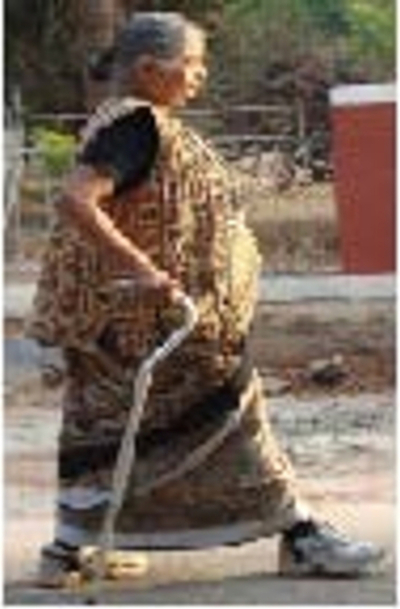
\includegraphics[scale=2.2]{images/086.jpg}
\end{figure}

\begin{thebibliography}{99}
%~ \rhead[\small \em The Role of Physical Exercise in Diabetes]{\small\thepage}
\bibitem{chap23–key01} Umpierre D, Ribeiro PA, Kramer CK, Leitao CB, et al. Physical\break activity advice only or structured exercise training and association with HbA1c levels in type 2 diabetes: A systematic review and meta–analysis. JAMA. 2011; 305 (17): 1790–9.
\bibitem{chap23–key02} Henriksen EJ. Effects of acute exercise and exercise training on insulin resistance. J Appl Physiol. 2002; 93 (2): 786–96.
\bibitem{chap23–key03} Manders RJ, Van Djik JW, \& van Loon LJ. Low–intensity exercise reduces the prevalence of hyperglycemia in type 2 diabetes. Med Sci Sports Exerc. 2010; 42 (2): 219–25.
\bibitem{chap23–key04} Snowling NJ \& Hopkins WG. Effects of different modes of exercise training on glucose control and risk factors for complications in type 2 diabetes patients: a meta–analysis. Diabetes Care. 2006; 29 (11): 2518–27.
\bibitem{chap23–key05} Helmrich SP, Ragland DR, Leung RW, \& Paffenbarger RS Jr.\break Physical activity and reduced occurrence of non–insulin–dependent diabetes mellitus. N Engl J Med. 1991; 325 (3): 147–52.
\bibitem{chap23–key06} Eriksson KF \& Lindgarde F. Prevention of type 2 (non–insulin–dependent) diabetes mellitus by diet and physical exercise. The 6–year Malmo feasibility study. Diabetologia, 1991; 34 (12): 891–8.
\end{thebibliography}

\newpage

%~ \rhead[\small \em \leftmark]{\small\thepage}
\chapter{Monitoring Diabetes – Recommended Tests and their Significance}\label{chap24}

Monitoring diabetes is an integral part of managing diabetes. It offers status updates about the current disease condition, and can help make predictions about the future disease course. Using this information, diabetics can successfully navigate through the maze of diabetes.

\noindent There are two main categories of monitoring tests:

\vspace{-\topsep}
\begin{enumerate}
\itemsep=0pt
\item Tests to evaluate blood glucose control
\item Tests to screen for complications of diabetes.
\end{enumerate}
\vspace{-\topsep}

\noindent{\textbf{Tests to evaluate blood glucose control}}

These tests are the main tools to check diabetes control, and mainly include blood tests. There are two types of blood tests available:

\vspace{-\topsep}
\begin{enumerate}[I.]
\itemsep=0pt
\item Tests to evaluate short–term diabetes control: These include\break finger prick method of home glucose monitoring and laboratory plasma glucose levels.
\item Tests to evaluate long–term diabetes control: These include HbA1c\index{HbA1C test} and fructosamine test\index{Fructosamine test}.
\end{enumerate}
\vspace{-\topsep}

\noindent\textbf{Tests to evaluate short–term glucose control}

These tests are usually recommended daily (in poorly controlled diabetes) or at least weekly. You should check your blood sugars at\break different times of the day, usually before food, but sometimes after food as well. The results tell you how well your treatment plan is\break working. Since the target blood glucose levels when patients are\break fasting (\textless  126 mg/dL) and after food (\textless  180 mg/dL by 2 hours) are well known, these tests tell you how close you are to these targets. In fact you should compile a log of the blood glucose levels measured at diffe\-rent times of the day and study the trend. If you find out that you are not at target, you can make the necessary changes in your daily routine to attain these goals. These measures include diet, physical exercise and medications. These blood tests can also tell you how your blood sugars respond to changes you make in your diet, physical activity and medications. Thus, you can fine–tune all these essential ingredients of good glucose control to achieve the recommended blood glucose\break levels. Just like a fine dining chef frequently tastes his dish to find out if it needs more salt or masala, you must check your blood sugar level frequently to see if you need to eat less, or exercise more, or increase the dose of your medication.

\noindent\textbf{How can you test blood glucose levels?}

Nowadays blood glucose meters are universally available, and are manufactured by many companies (Roche, Bayer, Johnson \& Johnson, Abbott, etc). You can buy any one of these meters and check your blood sugars.

You could also go to the laboratory recommended by your physician to have your plasma glucose level tested.

\noindent\textbf{When is there a need to check blood sugars more frequently?}

It is important to monitor blood sugar levels very closely in the following situations:

\vspace{-\topsep}
\begin{enumerate}[•]
\itemsep=0pt
\item Periods of increased stress on the body– infections, injury, surgery, emotional stress, etc
\item During pregnancy (if the woman is a diabetic)
\item When changes are made in diabetes medications
\item When taking certain medications like steroids that are known to cause increased blood sugar levels. It is also your physician’s responsibility to alert you about this issue.
\end{enumerate}
\vspace{-\topsep}

\noindent\textbf{Tests to evaluate long–term blood glucose control}

\noindent There are two tests available for this purpose:

\vspace{-\topsep}
\begin{enumerate}[i.]
\itemsep=0pt
\item HBA1c\index{HbA1C test}
\item Fructosamine test.\index{Fructosamine test}
\end{enumerate}
\vspace{-\topsep}

\noindent\textbf{The HbA1c test}

HBA1c test is also called glycated hemoglobin test, HbA1c, or\break simply A1c. It assesses the average blood glucose level over a three–month period.

Glycosylated hemoglobin forms when excess glucose attaches\break itself to hemoglobin (a substance in red blood cells) in the circulation. The average life\-span of a red blood cell is about 120 days or 3 months. Hence HBA1c provides a 3–month average of blood sugar levels. The higher your blood glucose levels were over the past ninety–day period, the higher your percentage of glycosylated hemoglobin will be.

The ADA recommends that an A1c be performed at least twice\break annually, and up to four times a year for individuals who are\break undergoing adjustments to treatment, or failing to meet treatment\break goals. Patients who use insulin to control their type 1 or type 2 diabetes\break should have the test performed quarterly as well.

A1c levels are the best measure of long term blood sugar control. While home monitoring by the finger–prick method provides a single snapshot of the blood sugar at a particular point in time, an A1c test is like a surveillance camera running continuously for three months, day and night, giving you a more comprehensive picture of average blood glucose levels.

The Diabetes Control and Complications Trial (DCCT), demonstra\-ted that people with type 1 diabetes were 40 to 75\% less likely to\break develop neuropathy, retinopathy, and nephropathy (kidney di\-sease) when they kept their A1c value at an average of 7.2\%. Follow–up\break studies of DCCT participants 6 years after the original study found that tight blood glucose control reduced the risk of atherosclerosis. Athero\-sclerosis is the main cause for majority of the complications of diabetes.

Similarly, the United Kingdom Prospective Diabetes Study (UKPDS) found that participants with type 2 diabetes who kept their A1c values below 7.0\% had a 25\% reduction in the incidence of complications. And for every percentage point decrease in HbA1c achieved, there was a 35\% reduction in the complication risk. Thus HBA1c levels not only a look back at the past three months, but provide a glimpse into your future risk of complications.

\vskip 3pt

\noindent\textbf{How accurate the HbA1c test?}

Certain situations can affect the results of the HbA1c test. Patients who are taking vitamin C and E, narcotic medications (like morphine, codeine, etc), and salicylates like aspirin can influence results of some A1c tests. Conditions such as iron deficiency anemia and chronic\break alcoholism can also affect the accuracy of the test. But in general this is a very reliable test.

\vskip 3pt

\noindent\textbf{Fructosamine test\index{Fructosamine test}}

This is another test that averages your blood sugar over a period of time (two to three weeks, as opposed to the 3–month average with the HbA1c test). The fructosamine test is a measurement of glycated serum proteins. Unlike HBA1c, where we measure glucose attached to hemoglobin, in the fructosamine test, we measure the excess sugar attached to proteins. The average lifespan of protein in the human body is about 14 to 21 days. Hence this test gives us the average blood sugar level over 2 to 3 weeks. It may be used as a companion to HbA1c when you want to find out how blood glucose control has responded to treatment changes over the past few weeks.

\clearpage

Fructosamine tests are available as home testing kits, but they\break should not be considered a replacement for daily glucose monitoring or HbA1c tests.

\noindent\textbf{Urine glucose test}

Available as reagent “dipstick” test, urinary glucose tests were once the standard method of measuring glucose levels at home for people with diabetes. But with the advent of accurate blood test–based home monitoring systems, urine glucose tests are now rarely used. Urine–based tests have several drawbacks.

\vspace{-\topsep}
\begin{enumerate}
\itemsep=0pt
\item Urine sugar tests are time–delayed. Glucose in the urine is seve\-ral hours old. The kidneys filter blood gradually to form drops of urine, which collect in the bladder drop–by–drop, waiting to come out when we decided to urinate. Hence glucose in urine is not a reflection of how much glucose is in the blood currently, but rather, how much glucose existed in the blood several hours ago.
\item Urine–based test is also not very sensitive or specific; a negative urine test only means that your blood glucose level is below 180 mg/dl.
\item If you have hypoglycemic unawareness, or are prone to frequent blood sugar lows, it is critical that blood monitoring be used\break instead of urine monitoring, as urine glucose testing cannot\break detect low blood glucose.
\end{enumerate}
\vspace{-\topsep}

Since urine tests are relatively inexpensive, patients who cannot afford blood–monitoring supplies may prefer urine glucose tests.\break Patients who cannot or will not prick themselves for home blood\break glucose monitoring due to discomfort or other reasons may find urine glucose tests preferable over blood glucose monitoring.

\noindent{\large\textbf{Test to screen for complications of diabetes}}

We have already discussed the ten devastating or debilitating\break complications that can be caused by diabetes. Monitoring diabetes also involves screening diabetics to identify people at risk for these\break complications, so that appropriate steps can be taken to prevent them in a timely manner.

\noindent\textbf{Tests to screen for cardiovascular complications (coronary artery disease, high cholesterol, high blood pressure)}

\noindent\textbf{a) Blood pressure\index{Blood pressure}}

Blood pressure should be checked at every clinic visit, and if\break found to be elevated on more than two occasions, treatment should be ini\-tiated to maintain blood pressure below 130/80 mm Hg.

\noindent\textbf{b) ECG (EKG) or electrocardiography\index{ECG or Electrocardiography}}

This is a tool of remarkable importance to identify a cardiac\break ailment. This is a record of the electrical activity of the heart. Ab\-normalities in this electrical pattern can alert the doctor to abnorma\-lities of the heart muscles that may be seen with coronary artery\break disease. This test should be performed at least once a year since not all diabetics with heart disease will have symptoms such as chest\break pain. If there are any abnormalities on the ECG, further heart testing is required in the form of cardiac stress tests and echocardiograms. These tests are explained in chapter \ref{chap12}.

\noindent\textbf{c) Lipid profile\index{Lipid profile}}

This should be checked annually. A fasting lipid profile is a blood test that assesses your risk for developing cardiovascular complications by measuring levels of total cholesterol, high–density lipoprotein (HDL or “good”) cholesterol, triglycerides, and low–density lipoprotein (LDL or “bad”) cholesterol\index{Low-density lipoprotein (LDL) cholesterol}.

It is also used to diagnose “diabetic dyslipidemia”\index{Diabetic dysplipidemia}, a condition\break characterized by high triglyceride and low HDL cholesterol\index{HDL cholesterol} levels that is common in type 2 diabetes and increases the overall risk of heart disease (For more information see chapter – \ref{chap13B}).

{
\begin{table}[H]
\centering
\caption*{\textbf{Cholesterol Goals Recommended for Adults with Diabetes}}
\small\addtolength{\tabcolsep}{-3pt}
\begin{tabular}{|c|l|l|l|}
\hline
 & & \,\,\textbf{NCEP* III Guidelines} & \,\,\textbf{ADA** Guidelines}\\
\hline
1. & HDL & \textgreater 40-60 mg/dl & \textgreater 40 mg/dl (men)\\
\hline
2. & LDL & \textless 100 mg/dl & \textless 100 mg/dl\\
\hline
3. & Triglycerides & \textless 150 mg/dl & \textless 150 mg/dl\\
\hline
\end{tabular}
\end{table}
\begin{quote}
* The National Cholesterol Education Program

** Standards of Medical Care for Patients with Diabetes Mellitus: ADA
Position Statement, 2013
\end{quote}
}\relax

\noindent\textbf{Tests to screen for kidney–related complications}

\textbf{a) Testing for Proteinuria}

Since a damaged kidney leaks protein into urine as explained in chapter \ref{chap14}, screening for diabetes induced kidney damage naturally includes checking for the presence of protein in urine. There are two tests for this purpose. One is to have the patient collect all the urine produced in a 24–hour period and checking for presence of protein in this urine sample, and then also measuring the total amount of protein in the urine.

Another easier way is to collect a single sample of urine, and by\break using a formula known as the albumin–to–creatinine ratio, estimate the amount of protein (or albumin) in the urine. This is an accurate and established method, and is much easier for patients and physicians. Presence of more than 30 mg/day is considered abnormal. A level between 30 mg and 300 mg of albumin in urine per day used to be called microalbuminuria.

\noindent Urine albumin levels should be checked as follows:

\vspace{-\topsep}
\begin{enumerate}[•]
\itemsep=0pt
\item In type 1 diabetics, 5 years after diagnosis, and annually thereafter
\item In type 2 diabetics, at times of diagnosis, and annually thereafter.
\end{enumerate}

\clearpage

\textbf{b) Serum creatinine\index{Serum creatinine} and eGFR}

Serum creatinine levels may also be measured to asses kidney\break function. Creatinine is a waste product produced by muscle meta-\break bolism. It is filtered out of the blood stream by the kidneys. If the kidneys are healthy, the creatinine level in the blood should be low, and\break creatinine level in the urine should be high. But if the kidneys are not working well, then creatinine level in the blood will rise.

Creatinine blood levels greater than 1.2 mg/dl in women and 1.4 mg/dl in men points to inadequate filtering by the kidneys (renal\break impairment).

Creatinine levels in the blood are also used to estimate GFR or glome\-rular filtration rate\index{Glomerular filtration rate (GFR)}. Normal GFR value is 90–125 ml/min/1.73 m2. When this level falls to 15 ml/min/1.73 m2, then the patient needs dialysis to stay alive.

\noindent\textbf{Comprehensive eye exam}

Diabetes damages the blood vessels in the retina, resulting in a\break condition known as diabetic retinopathy\index{Diabetic retinopathy}, which can lead to blindness.

Both the American Diabetes Association (ADA) and the National Eye Institute recommend an annual dilated–eye exam for people with diabetes. In a dilated–eye exam, eyedrops are used to counteract the normal reflex of the pupil to shrink in bright light. The ophthalmo\-logist uses a high–intensity focused light called a slit–lamp to illuminate the eye. Dilation opens up the pupil, allowing the ophthalmo\-logist to view the back, or fundus of the retina, and the blood vessels and\break optic nerve situated there.

An intraocular pressure test, also called a tonometry test\index{Tonometry test}, is used to screen for glaucoma\index{Glaucoma}. It involves blowing a quick puff of air onto the eye and measuring the resistance it meets. Another type of test uses fluoresceing dye to temporarily color the cornea before a tonometer is placed against the eye to measure fluid pressure. To avoid discomfort, anesthetic drops are placed on the eye beforehand.

\noindent Other parts of a comprehensive eye exam may include:

\vspace{-\topsep}
\begin{enumerate}[•]
\itemsep=0pt
\item Visual acuity test
\item Visual field test
\item Binocular test
\item Evaluation of your prescription eyeglasses or contacts, if you are\break required to use these.
\item Current ADA recommended schedule for dilated eye–exams are as follows:
\item For type 1 diabetics, starting 5 years after diagnosis, and annually thereafter
\item For type 2 diabetics, starting at the time of diagnosis, and annually thereafter
\item If you already have an eye disease, you may require more frequent assessment to monitor treatment and disease progression.
\end{enumerate}
\vspace{-\topsep}

\noindent\textbf{Tests to screen for neuropathy\index{Neuropathy}}

Inexpensive tests such as the monofilament test and tuning fork test can be done to screen for neuropathy. These tests evaluate the sensations of fine touch, pain and vibration.

\noindent The recommended testing schedule is as follows:

\vspace{-\topsep}
\begin{enumerate}[•]
\itemsep=0pt
\item For type 1 diabetics, starting 5 years after diagnosis, and annually thereafter.
\item For type 2 diabetics, starting at the time of diagnosis, and annually thereafter.
\end{enumerate}
\vspace{-\topsep}

\noindent\textbf{Tests to screen for diabetic foot}

Simple and inexpensive tests start with a visual inspection of the foot. Then the physician examines the strength of the pulse in the foot by feeling it. In addition, tests are done to detect what is known as Loss of Protective Sensation (LOPS). These again include very simple tests such as:

\vspace{-\topsep}
\begin{enumerate}[•]
\itemsep=0pt
\item Monofilament test
\item Tuning fork test
\item Vibration perception threshold test.
\end{enumerate}
\vspace{-\topsep}

This assessment should be done during every clinic visit or at least annually.

\noindent\textbf{Ketones\index{Ketones} and diabetic ketoacidosis\index{Diabetic ketoacidosis}}

Ketones are formed when the body cannot use insulin to process glucose into fuel and is forced to burn fat for energy. Trace amounts of ketones are not unusual and are usually no cause for alarm, but when accompanied by elevated blood sugars in high enough levels,\break ketones can trigger diabetic ketoacidosis (DKA), a potentially fatal\break medical emergency. DKA usually occurs in situations where someone has stopped taking required insulin injections; is taking an insufficient dose of insulin; or is taking contaminated, expired, or otherwise bad\break insulin. The physical stress of a flu, cold, or other illness usually\break increases both blood glucose levels and the need for insulin, and DKA often occurs in these situations.

Although people with type 1 diabetes are much more prone to DKA, type 2 diabetics are at risk as well.

\noindent\textbf{When should we check for ketones?\index{Ketones}}

If your blood glucose level is 250 mg/dl or higher on two or more consecutive readings, you should check for ketones in the urine.

There is a urine test for ketones that can be used at home. The test uses a chemically treated reagent strip (Ketostix) that is dipped in a urine sample to check for the presence of ketones. The strip changes color and the color is matched to an enclosed chart that indicates the presence and level of ketones in the urine.

\noindent{\textbf{Summary}}

The following two tables summarize all the tests discussed in this chapter so far.

{
\begin{center}
\centering
\small\addtolength{\tabcolsep}{-3pt}
\begin{tabular}{|l|l|l|}
\hline
\multicolumn{1}{|c|}{\textbf{Tests of blood}}  & \multicolumn{1}{c|}{\textbf{Frequency of}} & \multicolumn{1}{c|}{\multirow{2}{2.8cm}{\textbf{Purpose of testing}}}\\
\multicolumn{1}{|c|}{\textbf{glucose control}}  & \multicolumn{1}{c|}{\textbf{testing}} & \\
\hline
\textbf{Pin prick method} & Daily to weekly & To assess short-term\\
\textbf{of home glucose} &  & blood glucose control\\
\textbf{monitoring} &  & To assess effect of diet,\\
 &  & exercise and medications\\
 &  & on blood glucose\\
\hline
\textbf{HBA1c} & Every 3 months & To assess long-term\\
 &  & blood glucose control\\
\hline
\textbf{Fructosamine} & Every 2-3 weeks & To assess short-term\\
 &  & changes in blood glucose\\
 &  & when starting new\\
 &  & therapies, etc\\
\hline
\end{tabular}
\end{center}
}\relax

\vskip 8pt

\begin{center}
\textbf{\textit{TESTS TO SCREEN FOR COMPLICATIONS OF DIABETES}}
\end{center}

\vskip -.5cm

{
\small\addtolength{\tabcolsep}{-5pt}
\begin{longtable}{|l|l|l|l|}
\hline
\multicolumn{1}{|c|}{\textbf{Complication}} & \multicolumn{1}{c|}{\textbf{Test(s)}} & \multicolumn{1}{c|}{\textbf{Purpose}} & \multicolumn{1}{c|}{\textbf{Frequency}}\\
\hline
\textbf{Hypertension} & Blood pressure & Evaluate BP & Every clinic\\
 & check & changes & visit\\
\hline
\textbf{Cholesterol} & Fasting serum & Assess lipid & At least\\
\textbf{abnormalities} & lipids & levels & annually\\
\hline
\textbf{Coronary artery} & ECG & Evaluate heart & Annually\\
\textbf{disease, congestive} & Chest x-ray in & muscle function & \\
\textbf{heart failure} & some cases &  & \\
\hline
\textbf{Nephropathy} & Urine albumin & Identify & Annually\\
 & Serum creatinine & nephropathy in & \\
 & eGFR & its early stages & \\
\hline
\textbf{Retinopathy} & Dilated-eye exam & Identify & Annually\\
 &  & retinopathy early & \\
 &  & by examining & \\
 &  & the retina & \\
\hline
\textbf{Neuropathy} & Pinprick test & Evaluate & Annually\\
 & Monofilament test & sensations of & \\
 & Tuning fork test & fine touch, pain & \\
 &  & and vibration to & \\
 &  & identify early & \\
 &  & signs of & \\
 &  & neuropathy & \\
\hline
\textbf{Diabetic foot} & Pinprick test & To identify the & Every clinic\\
 & Monofilament test & foot at risk for & visit, and at\\
 & Tuning fork test & complications & least annually\\
 & Vibration perception & due to nerve & \\
 & threshold test & damage and & \\
 & Strength of pulse & poor blood & \\
 & in foot & supply & \\
\hline
\end{longtable}
}\relax


\chapter{Prevention of Diabetes}\label{chap25}

So far in this book we have discussed the multiple adverse effects of\break the disease, its causes, and its treatment. But since “prevention is\break better than cure”, any book about diabetes is incomplete without\break talking about prevention. You will be pleasantly surprised to know that diabetes and its complications can be prevented!

Medical science has made tremendous progress, especially over the last decade. As a result we are now capable of preventing diabetes and its complications at 3 levels, namely:

\vspace{-\topsep}
\begin{enumerate}
\itemsep=0pt
\item Primary prevention
\item Secondary prevention
\item Tertiary prevention.
\end{enumerate}
\vspace{-\topsep}

\noindent{\textbf{Primary prevention of diabetes}}

This refers to measures aimed at preventing a person from getting diabetes in the first place. This is without doubt the grandest dream as well as the biggest hurdle for the medical community and the country as a whole.

Several studies have shown that some diabetes drugs may have the potential to delay or prevent type 2 diabetes. Metformin reduced the risk of type 2 diabetes by 31\% in the Diabetes Prevention Program (DPP), acarbose reduced the risk by 32\% in the STOP–NIDDM trial.

\noindent\textbf{How can this be achieved?}

The first step is to identify people at risk for developing diabetes. People who have ‘prediabetes’\index{Prediabetes} are up to 15 times more likely to develop diabetes within 10 years if no preventive actions are undertaken. This risk is much higher among Indians compared to Caucasians.

\noindent\textbf{Prediabetes is diagnosed if:}

\vspace{-\topsep}
\begin{enumerate}[•]
\itemsep=0pt
\item The fasting blood sugar level is between 100 to 125 mg per deci\-li\-ter– this is termed Impaired Fasting Glucose (IFG)\index{Impaired fasting glucose (IFG)}.
\item A 2–hour blood sugar level is between 140 to 200 mg per deciliter after the OGTT (oral glucose tolerance test)\index{Oral glucose tolerance test (OGTT)} – this is termed impaired glucose tolerance (IGT).
\end{enumerate}
\vspace{-\topsep}

\noindent\textbf{But who should be tested to find out if they have prediabetes?}

Obviously it is not practical or economically feasible to test everyone. The following individuals are at high risk for developing diabetes, and should be tested for prediabetes:

\vspace{-\topsep}
\begin{enumerate}[•]
\itemsep=0pt
\item Age above 25–30 years in case of Indians (45 years for Caucasians)
\item Family history of diabetes
\item Personal history of hypertension
\item Personal history of high cholesterol
\item Obesity
\item Sedentary lifestyle
\item Women who had a gestational diabetes while they were pregnant.
\end{enumerate}
\vspace{-\topsep}

\noindent\textbf{What if the fasting glucose level and post–prandial glucose levels are normal?}

As per current recommendations, these tests should be repea\-ted every 2–3 years.

\noindent\textbf{Preventive Interventions in Prediabetics}

The next part of the puzzle is if and how we can prevent the\break onset of diabetes in this high–risk group of prediabetics. For long we watched helplessly as these individuals fell victim to diabetes. But in 2002, based on several small studies that had demonstrated the bene\-fit of diet and exercise in preventing or delaying diabetes, a landmark study was under\-taken in the United States of America. The study\break enrolled 3234 prediabetic patients from 27 major medical centers and divided them into 3 groups.

\vspace{-\topsep}
\begin{enumerate}[•]
\itemsep=0pt
\item The first group called the lifestyle group received intensive\break training in diet, physical activity, and behavior modification. The indi\-viduals in this group exercised for 150 minutes per week, and cut their intake of fat and excess calories. The goal was a 7\% reduction in body weight.
\item The second group was treated with metformin.
\item The third group was treated with placebo pills.
\end{enumerate}
\vspace{-\topsep}

The results of these interventions have become a game changer in our crusade against diabetes.

\vspace{-\topsep}
\begin{enumerate}[•]
\itemsep=0pt
\item Lifestyle intervention reduced the risk of diabetes by 58\%. In fact, in prediabetics older than 60 years, the risk was reduced by 71\%.
\item For every kilogram of weight reduction, the risk of diabetes fell by 16\%!
\item Metformin treatment also reduced diabetes risk by 31\%.
\end{enumerate}
\vspace{-\topsep}

The question, however, is if this benefit is durable. A follow–up study done 10 years later showed that the lifestyle intervention group continued to have a 34\% decreased risk of developing diabetes, and the metformin group had an 18\% decreased risk.$^{\text{\cite{chap25–key01}}}$

However only 4.4\% of the 3243 prediabetics in this study were\break Indians. To overcome this demographic limitation a study was done in India involving 531 patients with prediabetes. It showed that lifestyle interventions (diet and exercise) decreased the risk of diabetes by\break 28.5\%. Metformin therapy decreased diabetes risk by 26.4\%.$^{\text{\cite{chap25–key02}}}$

Similar encouraging results have been seen in studies done around the world (Finland, China, Japan, etc).

Another study done in women who had gestational diabetes while pregnant showed a 50\% reduction in diabetes as a result of intense lifestyle measures and metformin therapy.$^{\text{\cite{chap25–key03}}}$

\vskip 6pt

\noindent\textbf{The fantastic work done over the past decade has made the\break following facts clear:}

\begin{enumerate}[•]
\itemsep=0pt
\item Diabetes can be prevented in individuals at high risk of developing diabetes (prediabetics).
\item Lifestyle changes (150 minutes of exercise per week and diet) aimed at weight loss is the best intervention to prevent diabetes.
\item Metformin therapy can also prevent diabetes but not to the same extent as lifestyle intervention.
\end{enumerate}

\noindent\textbf{Secondary prevention of diabetes}

This refers to efforts aimed at early diagnosis and treatment of dia\-betes. This applies to people who have unfortunately already crossed over from prediabetes to diabetes.

Secondary prevention is important because many are unaware of their disease state and are undiagnosed. But this ignorance is no bliss, since the high sugar levels silently destroy the body from within. Early diagnosis and treatment can prevent this destruction, and ensure a long and healthy life.

\vskip 6pt

\noindent{\textbf{Tertiary prevention of diabetes}}

Tertiary preventive measures are aimed at preventing complications of diabetes. These include both acute complications (diabetic\break ketoacidosis, hyperglycemic coma, hypoglycemia due to treatment), and chronic complications.

As explained throughout this book, the key to preventing diabetic complications is tight glucose control.

Thus, you will be heartened to know that diabetes can be tackled at every stage, including – and most importantly – even before it occurs!

\begin{thebibliography}{99}
\bibitem{chap25–key01} Diabetes Prevention Program Research Group, Knowler WC, Fowler SE, Hamman RF, et al. 10–year follow–up of diabetes\break incidence and weight loss in the Diabetes Prevention Outcomes Study. Lancet. 2009; 374 (9702): 1677–86.
\bibitem{chap25–key02} Ramachandran A, Snehalatha C, Mary S, Mukesh B, et al. The\break Indian Diabetes Prevention Programme shows that lifestyle\break modification and metformin prevent type 2 diabetes in Asian Indian subjects with impaired glucose tolerance (IDPP–1).\break Diabetologia. 2006; 49 (2): 289–97.
\bibitem{chap25–key03} Ratner RE, Christophi CA, Metzger BE, Dabelea D, et al. Prevention of diabetes in women with a history of gestational diabetes: Effects of metformin and lifestyle interventions, J Clin Endocrinol Metab. 2008; 93 (12): 4774–9.
\end{thebibliography}


\chapter{Treating Diabetes – Oral Medications and Insulin}\label{chap26}

A commonly asked question by our patients is “Doctor, I will follow dietary instructions and exercise, can I postpone or avoid taking medi\-cations?”

This is a more complicated question than most people realize.\break Many factors have to be taken into consideration in order to answer this question. The main consideration is whether you have type 1 or type 2 diabetes. Type 1 diabetics cannot survive without medications. Type 1 diabetics produce no insulin in their bodies. Without insulin it is\break impossible to stay alive with type 1 diabetes. Diet and exercise can help reduce the total insulin requirement.

But if a type 2 diabetic asks this question, then the answer is “yes and no”! If a person is newly diagnosed with diabetes, it is possible to keep blood sugar under control by reducing weight, eating healthy food and exercising. Unfortunately such patients are only a mino\-rity. According to the Center for Disease Control (CDC), only about 17\% of American adults are able to control their diabetes by diet and\break exercise alone. In fact, majority of patients with type 2 diabetes require medications to keep their blood sugars under control. Time and again in this book we have talked about the importance of controlling blood glucose levels in preventing the myriad complications of diabetes. In diabetes, the ends are more important than the means. Medications are an important means of achieving the ultimate goal of good glucose control.

\clearpage

\noindent\textbf{What are the currently available treatment options for diabetics?}

There are two main types of treatments for diabetes: insulin\break injections and oral medications. For type 2 diabetes, which is almost 95\% of all diabetes, oral medications are the mainstay of drug\break therapy. Hence, we will first discuss oral medications and then talk about insulin in this chapter.

\vskip 6pt

\noindent\textbf{What are the different oral medications available for therapy of type 2 diabetes?}

As of now, there are seven main classes of oral medications for type 2 diabetes:

\vspace{-\topsep}
\begin{enumerate}[•]
\itemsep=0pt
\item Biguanides
\item Sulfonylureas
\item Glitazones
\item Alpha–glucosidase inhibitors
\item Meglitinides
\item DPP–4 Inhibitors
\item SGLT$_{\text{2}}$ Inhibitors
\end{enumerate}
\vspace{-\topsep}

A new medication called canagliflozin (brand name Invokana)\break belonging to the class of medications called SGLT2 inhibitor (sodium–glucose co–transporter 2 inhibitor) has been recently approved by the FDA for use in type 2 diabetes, and can be used alone or in combination with other diabetes medications.

Each class of medication works in a slightly different way. We will now review each of these medications.

\vskip 6pt

\textbf{Biguanides}

\textbf{Drugs in this group:} Metformin

\textbf{Brand names in India:} Melmet, Glyciphage, Glycomet etc.

\textbf{Brand names in USA:} Glucophage

\noindent\textbf{The history of Metformin}

Metformin has an interesting history. It was derived by chemi\-cally modifying a compound called guanidine, which was isolated from a plant called French lilac. In fact, this plant was used in the Middle Ages to treat diabetes, but now we know that this plant is poiso\-nous! Scie\-ntists were able to modify the chemical to overcome its poisonous properties. In the 1950s, metformin was being used to treat flu because it was thought it had antiviral properties. But it was inci\-de\-ntally found to cause hypoglycemia! This generated interest in its anti–diabetic properties.

Metformin is often preferred over sulfonylureas because it does not cause significant hypoglycemia, and nor do they promote weight gain. They have also been shown to have a positive effect on blood lipid levels.

Metformin is prescribed two to three times daily with meals. The extended release version is designed for once–a–day use, usually with an evening meal. It may also be used in conjunction with a sulfonylurea drug or with insulin therapy.

\noindent\textbf{How does metformin work in the body?}

Metformin works by decreasing the amount of glucose your liver releases into the blood, and in addition facilitating the utilization of insulin. It promotes weight loss, improves the cholesterol profile, and reduces insulin resistance. The United Kingdom Prospective Diabetes Study (UKPDS), a landmark 20 year clinical study, found that overweight patients treated with metformin experienced a significantly lower mortality rate than those treated with sulfonylurea drugs,\break and had a marked reduction in strokes and heart attacks. The ADA\break recommends metformin be used as the 1st line therapy in type 2\break diabetes. It is a relatively cheap medication, and is very popular in developing and underdeveloped nations in particular.

\clearpage

\noindent\textbf{Possible side effects of metformin}

If not for its side effects, metformin would have been the gold\break standard drug for diabetes. Metformin is not recommended for\break people with kidney or liver problems due to the risk of lactic acidosis, a rare but potentially fatal buildup of lactic acid in the bloodstream that\break occurs when the liver and kidneys do not adequately remove lactic acid. Signs of lactic acidosis include weakness, fatigue, dizziness, brea\-thing problems, and unexplained muscle and/or stomach pain. If you experience any of these symptoms while taking metformin, seek\break immediate medical attention.

Biguanides are also not recommended for use in patients with\break congestive heart failure. Other potential side effects of metformin\break include:

\vspace{-\topsep}
\begin{enumerate}[•]
\itemsep=0pt
\item Gastrointestinal distress (gas, diarrhea and gastric irritation)
\item Nausea
\item Metallic taste in the mouth
\item Depletion of vitamin B12 with long–term use
\end{enumerate}
\vspace{-\topsep}

\textbf{Sulfonylureas}

\textbf{Drugs in this group:} Gipizide, Glimepiride, Glyburide

\textbf{Brand names in India:} Amaryl, Diapride, Glynase, Dibizide, etc.

\textbf{Brand names in USA:} Glucotrol, Amaryl, Glynase

\vskip 3pt

There is an interesting story behind the discovery of this group\break of medications. In 1942 a French doctor, Marcel Janbon and his\break colleagues were treating typhoid patients with sulfonamide (a sulfa anti\-biotic). They noticed that these patients were experiencing severe hypoglycemia. By 1946, it was confirmed by laboratory experiments that the cause for the hypoglycemia was the sulfa drug, which was\break directly stimulating insulin secretion. It was not long before these drugs began to be used as anti–diabetics! Introduced in the 1950s, the oldest sulfonylureas or first generation drugs are now obsolete. We now use the newer, or second–generation sulfonylureas. They are\break much more potent and are typically prescribed at daily dosages\break ranging from 1 to 4 milligrams. The newer drugs are usually taken twice daily before meals, and extended–release medications can be\break taken once daily. Your doctor will tell you when and how often to take your medication. Whatever the schedule, you should always try to take it consistently at the same time everyday.

\vskip 4pt

\noindent\textbf{How do \textit{sulfonylureas\index{Sulfonylurea}} work?}
\vskip 4pt

They are called “secretogogues”, as they cause the pancreas to\break release or secrete more insulin, which in turn lowers the blood\break glucose level. Conversely, sulfonylureas may not be effective in\break people with long–standing diabetes who have lost most or all of their pancreatic beta cell function.

In addition, drugs such as glimepiride, which is the newest of the sulfonylurea drugs, also work to decrease insulin resistance by binding with insulin receptors. So in addition to increasing insulin output, this drug also allows the body to utilize the insulin more effectively.

\vskip 4pt

\noindent\textbf{What are the important side effects of this class of medicines?}
\vskip 4pt

The most serious potential side effect of sulfonylurea drugs is\break hypoglycemia, or low blood sugar. The older sulfonylureas in parti\-cular, are more likely to cause this reaction if they are taken along with other medications.

Another vexing issue can be weight gain. This can prove counter\-productive since weight gain will work against the benefits of the drug by increasing insulin resistance. Your physician may prefer to use\break a newer sulfonylurea if you are overweight. Sulfonylureas are not\break pre\-ferred in older individuals.

\vskip 6pt

\textbf{Generic Glitazones\index{Glitazones} (Insulin sensitizers)}
\vskip 3pt

\textbf{Drugs in this group:} Pioglitazone

\textbf{Brand names in India:} Pionorm, Pioz, etc.

\textbf{Brand names in USA:} Actos, Avandia

\vskip 5pt

\noindent\textbf{How do glitazones\index{Glitazones} work?}
\vskip 3pt

Glitazones are insulin sensitizers. They are also called thiazolidinediones(TZDs). They target the insulin receptors in muscle and fat cells to increase insulin sensitivity in the body. They also reduce glucose production. They can be effective in lowering blood pressure and\break triglyceride levels, and in increasing HDL (or “good”) cholesterol.\break Because they lower glucose so effectively, they also reduce hyper\-insu\-linemia (excess circulating insulin).

ADA recommends Glitazones as second line drugs in type 2\break diabetes.

\vskip 5pt

\noindent\textbf{Possible side effects of glitazones\index{Glitazones}}

Because of the association between glitazones and liver failure, the FDA (Food and Drug Administration, USA) has imposed strict guidelines on assessing liver function in patients taking these drugs. If you take a glitazone, you must have regular testing of the liver function (specifically a test called ALT). Liver tests should be done before treatment starts, and every two months for the first year you are taking the drug, and as recommended by your doctor thereafter (usually at least once in 3–6 months). The drug should not be started in patients who have ALT levels that are greater than 2.5 times higher than the normal upper limit. The drug should be discontinued if ALT levels increase to more than 3 times the normal upper limit.

These drugs can also either cause or worsen congestive heart\break failure (CHF), and hence should not be used in patients with CHF, and should be discontinued if patients develop CHF while on treatment with a drug in this class.

Due to the concerns about the risk of bladder cancer, glitazones were banned in India in July 2013. But this decision was reversed in August 2013 with a recommendation to include a warning about the drug’s potential bladder cancer risk.

\noindent Other side effects of TZD therapy may include:

\vspace{-\topsep}
\begin{enumerate}[•]
\itemsep=0pt
\item Edema (water retention) of the ankles or legs
\item Anemia
\item Weight gain
\item Muscle weakness
\item Headaches
\item Fatigue
\item Cold/flu–like symptoms.
\end{enumerate}
\vspace{-\topsep}

\textbf{Starch Blockers\index{Starch blocker}}

\textbf{Alpha–Glucosidase Inhibitors (AGI)\index{Alpha Glycosidase inhibitors (AGI)}}

\textbf{Drugs in this group:} Acarbose, Miglitol

\textbf{Brand names in India:} Diabose, Glycobay, etc.

\textbf{Brand names in USA:} Precose, Glyset

The alpha–glucosidase inhibitors are also called “starch blokers”. These medications must be taken at each meal with the first bite of food in order to be effective. AG inhibitors may be prescribed along with a sulfonylurea drug, metformin, or insulin.

Acarbose works by slowing digestion. More specifically, they block the enzymes responsible for the breakdown of carbohydrates in the intestine, so that blood glucose rise is slower and steadier. They may be prescribed for you if you have difficulty keeping your postprandial (after meal) blood glucose levels under control. These drugs may be a preferred therapy in overweight patients, since they do not promote weight gain like the sulfonylureas and glitazones.

Because of the way they work, most of the side effects of the AG\break inhibitors are gastrointestinal such as diarrhea, gas, and cramping.\break However, like metformin, the uncomfortable side effects can be greatly reduced by starting with a small dose and gradually increasing it as needed.

People with serious gastrointestinal disorders, including intestinal disease or obstructions, inflammatory bowel disease, and colonic\break ulceration, should not take AG inhibitors.

\textbf{Meglitinides}

\textbf{Drugs in this group:} Repaglinide and Nateglinide

\textbf{Brand names in India:} Eurepa, Novonorm, Reepag

\textbf{Brand names in USA:} Prandin, Starlix

Repaglinide and nateglinide are currently the only FDA–approved meglitinide class drugs. Like AG inhibitors, they are taken at meal times (usually about fifteen minutes before eating) to prevent a postprandial blood sugar rise. People who tend to develop high blood\break sugars after meals may benefit from treatment with meglitinide drugs. Repaglinide is also FDA–approved for use with the insulin sensitizers.

\vskip 4pt
\noindent\textbf{How do they work?}
\vskip 4pt

Meglitinides are short–acting oral hypoglycemic agents. They bind to the insulin–producing beta cells of the pancreas, and stimulate\break insulin secretion in response to the level of glucose in the bloodstream. Taken before a meal, meglitinides can boost what is known as first–phase insulin release, the production of insulin that is a response to the initial boost of carbohydrate–generated blood glucose after a meal.

\vskip 4pt
\noindent\textbf{Possible side effects of Meglitinides}
\vskip 4pt

Hypoglycemia and weight gain are the usual side effects.

\textbf{DPP–4 inhibitors}

\textbf{Drugs in this group:} Sitagliptin, Vildagliptin, Saxagliptin, Linag\-liptin.

\textbf{Brand names in India:} Galvus, Onglyza, etc.

\textbf{Brand names in USA:} Januvia, Onglyza, Trajenta


This newest class of oral anti–diabetes agents work by inhibi\-ting the actions of the enzyme DPP–4 (dipeptidyl peptidase–4). DPP–4\break inhibitors are used as an adjunct to diet and exercise. They improve blood glucose control in type 2 diabetes, and are useful both as mono\-therapy and as combination therapy with metformin or glitazones.

They can be taken once daily, with or without food. They are\break associated with a lower incidence of hypoglycemia. Based on your\break kidney function, your physician will put you on the right dose of this medication.

There is some concern that this class of medications can increase the risk of pancreatitis\index{Pancreatitis} (inflammation of the pancreas) and pancreatic cancer. The FDA in USA is reviewing this currently.

\textit{Teneligliptin} was introduced in India in May 2015. It has gained\break popularity and is widely used in type 2 diabetes as it is cost effective and efficacious.

\textbf{Brand names:} Tenepride, Tenepan, Ten DC Afogliptin etc.

\textbf{GLP–1 Agonists}

\textbf{Drugs in this group:} Exanetide, Liraglutide, Albiglutide, Taspo\-glutide, Lixisenatide

\textbf{Brand names in India:} Victoza

\textbf{Brand names in USA:} Byetta, Victoza



GLP–1 (Glucagon–like Peptide) is a naturally occurring hormone\break in our intestines. It stimulates insulin secretion from the pancreas in response to glucose. GLP–1 agonists are drugs that mimic these\break actions. This is the newest member of diabetes medications, and hence we have the least amount of safety data about it. For the same reason, this class of drugs is not recommended as first line therapy. Instead it is usually used as an add–on drug when patients with type 2 diabetes are not well controlled despite using first–line drugs such as metformin or sulfonylureas.



Possible side effects include nausea, pancreatitis, and renal failure. Hence they are contraindicated in patients with pre–existing kidney problems, or a history of pancreatitis.

\noindent{\textbf{Combination drugs}}

Combination drugs combine medications from two classes of drugs. Judicious combinations of two or more drugs with complimentary\break actions can act effectively to normalize blood glucose, when taking one drug alone does not bring down glucose levels adequately. While these drug combinations are usually more potent than using a single drug, the risk of side effects, especially hypoglycemia is also higher. Hence more caution needs to be exercised when using them.

\noindent{\textbf{So many choices, but where do I start?}}

It is comforting to know that there are many drug choices for type 2 diabetes, and it is exciting to note that there are more drugs in the pipeline, thanks to ongoing research and development across the globe. But when it comes to choosing the right first therapy for you, your physician will usually start with one drug, after evaluating several\break factors such as:

\vspace{-\topsep}
\begin{enumerate}[•]
\itemsep=0pt
\item Baseline weight of the patient (overweight or underweight)
\item The effect the chosen drug will have on patient’s weight
\item Risk of hypoglycemia
\item Cost
\item Side effect profile of drug
\item Other disease(s) patient has, and what effect the chosen drug may have on these conditions (like hypertension, high cholesterol,\break depression, kidney problems, liver problems, cardiac problems, etc)
\item Patient’s preference.
\end{enumerate}
\vspace{-\topsep}

\clearpage

In general, most patients are started on monotherapy with\break metformin, and in some cases a sulfonylurea. If after 3–6 months of using this drug at the maximum tolerated dose, the patient is unable to achieve the blood sugar goals, then a second agent is usually added (such as GLP–1 agonist). If patients continue to have high blood sugars, then it may be time to add insulin to the regimen. More often than not, type 2 diabetics will eventually end up needing insulin therapy due to the progressive nature of the disease (eventually there are not enough pancreatic beta cells left to produce insulin due to beta cell apoptosis or death).

\noindent{\textbf{The first few days and weeks after starting therapy: How can you avoid a bumpy ride?}}

It is but expected that patients feel overwhelmed when they are first diagnosed with diabetes. Before they can even overcome the shock of realizing that they have diabetes, they are expected to stick to a strict treatment regimen, be aware of the side effects of the drugs\break being prescribed, check their blood sugars regularly, and the list goes on!

There is only one way to deal with this situation, and that is to be systematic. The following tips will go a long way in helping a newly diagnosed diabetic navigate through the first few weeks:

\vspace{-\topsep}
\begin{enumerate}[•]
\itemsep=0pt
\item Note down the exact name of the medication prescribed, the dose, and the time of day you should take the medication.
\item Read the label on the medication box to familiarize yourself with its potential side effects.
\item If the instructions your doctor gave you and the instructions on the medication label do not match, then call your doctor to clarify before you take the medication.
\item Inform your family members and co–workers, so that they are aware of the ever–present–risk of hypoglycemia with diabetes medications.
\item Keep the medications in a safe place away from direct sunlight, heat or humidity, all of which can decrease the potency of the medication.
\item Keep the medications out of reach of children.
\item If women are pregnant or planning to become pregnant, they should not be taking these medications. So please inform your doctor if pregnant or planning to become pregnant.
\item Keep a logbook of your blood glucose levels. This will help in asse\-ssing how the medication is working for you.
\item Keep a source of quick glucose with you all the time, for that\break unexpected moment of hypoglycemia.
\end{enumerate}
\vspace{-\topsep}

\noindent{\textbf{Insulin\index{Insulin} in the treatment of Diabetes}}

Insulin is a polypeptide hormone, produced by pancreatic beta\break cells in the Islets of Langerhans. The discovery of insulin was the game–changer in diabetes. On 11$^{\text{th}}$ January 1922 insulin was used, till date, there is no medication more powerful than insulin. When all else fails, you can depend on insulin to save the day! It is nothing short of the legendary “\textit{Brahmasthra}”!

\noindent\textbf{Should every diabetic be treated with insulin?}

While not every diabetic needs insulin, it is a must in the following situations:

\vspace{-\topsep}
\begin{enumerate}[•]
\itemsep=0pt
\item Type 1 diabetes (since there is almost no insulin production in the body)
\item Pregnancy or gestational diabetes (since we do not wish to expose the growing fetus to any of the diabetes oral medications).
\end{enumerate}
\vspace{-\topsep}

\noindent\textbf{Should type 2 diabetes be treated with insulin? If so, when?}

Before the advent of oral anti–diabetic medications like metformin and sulfonylureas, insulin was the only available therapy for any type of diabetes. Insulin is in fact the best drug for both type 1 and type 2\break diabetes. But in general, due to many reasons such as convenience, personal reluctance, etc, oral medications are used as first–line\break therapy for type 2 diabetes. But insulin is definitely indicated in\break certain special situations as listed below:

\begin{enumerate}[•]
\itemsep=0pt
\item A newly diagnosed diabetic who has severely uncontrolled blood\break sugars
\vspace{-\topsep}
\begin{enumerate}[•]
\itemsep=0pt
\item Fasting sugar \textgreater  250 mg/dl
\item Postprandial sugar \textgreater  300 mg/dl
\item HBA1c \textgreater 9\%
\end{enumerate}
\item Type 2 diabetic who was previously doing well on oral anti–diabetic medications, but is no longer responding to maximum tolerable doses of oral medications
\item Type 2 diabetic who becomes pregnant
\end{enumerate}
\vspace{-\topsep}

Adding insulin may actually help preserve beta cell function and improve long–term glycemic control in type 2 diabetes.

\noindent\textbf{What are the current recommendations regarding insulin therapy among Indians?}

This is well summarized in the following algorithm.

\begin{figure}[h]
\centering
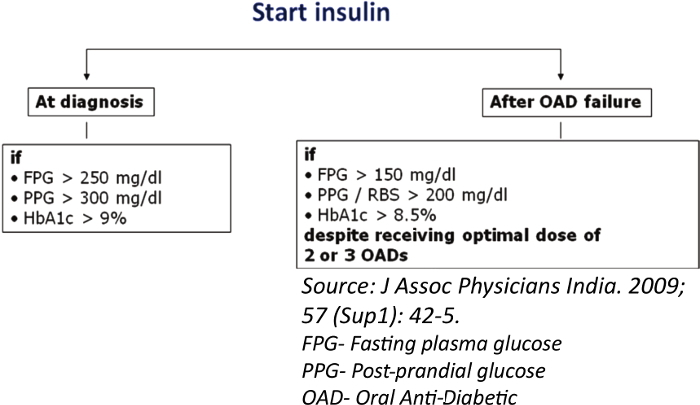
\includegraphics[scale=2.3]{images/087.jpg}
\end{figure}

\noindent\textbf{What are the different types of insulins available in this day and age?}

We currently use two main types of insulin preparations—human insulin and analog insulin. These two are again classified based on how fast or how slowly the insulin is absorbed into the body, and for how long it stays active inside the body.

\vskip 5pt

This classification is shown in the following table:

{
\begin{center}
\small\addtolength{\tabcolsep}{-1pt}
\begin{tabular}{|l|l|l|}
\hline
\multicolumn{1}{|c|}{\textbf{Onset and duration}} & \multicolumn{1}{c|}{\multirow{2}{2.3cm}{\textbf{Human Insulin}}} & \multicolumn{1}{c|}{\multirow{2}{2.3cm}{\textbf{Analog Insulin}}}\\
\multicolumn{1}{|c|}{\textbf{of action}} &  & \\
\hline
Rapid-acting & \quad\qquad- & Lispro, aspart, glulisine\\
\hline
Short-acting & Regular insulin & \qquad\qquad-\\
\hline
Intermediate-acting & NPH insulin & \qquad\qquad-\\
\hline
Long-acting & \quad\qquad- & Glargine, detemir\\
\hline
\end{tabular}
\end{center}
}\relax

\noindent\textbf{What is the difference between human insulin and analog insulin?}

Analog insulin is the newest preparation of insulin. It aims to mimic the action of natural insulin in the body as closely as possible, and thereby overcome some of the limitations of the older human insulin. The newer analog insulins have the following advantages over human insulin:

\vspace{-\topsep}
\begin{enumerate}[•]
\itemsep=0pt
\item The rapid–acting analog insulins are absorbed into the blood much faster than regular insulin. Also they have a shorter duration of\break action than regular insulin. Thus, they are quick and short, which is ideal to cover for the spike in blood glucose that is expected after a meal.
\item The long–acting analog insulins have a longer duration of action than NPH insulin (human insulin). Also the analog insulins are less likely to cause hypoglycemia.
\end{enumerate}
\vspace{-\topsep}

But as is the case with any new drug, analog insulins are much more expensive than human insulin. More importantly, since they are\break relatively new, we have less safety data on these newer preparations with regard to their side effects, etc.

The kinetics of all these different types of insulins are shown in the following tables:

\vspace{-\topsep}
{
\begin{center}
\small\addtolength{\tabcolsep}{-2pt}
\begin{longtable}{|l|l|l|l|}
\hline
\multicolumn{1}{|c|}{\textbf{Rapid and short-}} & \multicolumn{1}{c|}{\textbf{Onset of action}} & \multicolumn{1}{c|}{\textbf{Peak activity}} & \multicolumn{1}{c|}{\textbf{Duration of action}}\\
\multicolumn{1}{|c|}{\textbf{acting insulins}} & \multicolumn{1}{c|}{\textbf{(minutes)}} & \multicolumn{1}{c|}{\textbf{(minutes)}} & \multicolumn{1}{c|}{\textbf{(hours)}}\\
\hline
Insulin lispro & 15 & 30-70 & 2-5\\
\hline
Insulin aspart & 10-20 & 40-90 & 3-5\\
\hline
Insulin glulisine & 20 & 55 & Unknown\\
\hline
Regular insulin & 30-60 & 120-180 & 6-8\\
\hline
\end{longtable}
\end{center}
}\relax

{
\begin{center}
\small\addtolength{\tabcolsep}{-4pt}
\begin{tabular}{|l|l|l|l|}
\hline
\multicolumn{1}{|c|}{\textbf{Intermediate and}} & \multicolumn{1}{c|}{\textbf{Onset of action}} & \multicolumn{1}{c|}{\textbf{Peak activity}} & \multicolumn{1}{c|}{\textbf{Duration of action}}\\
\multicolumn{1}{|c|}{\textbf{long-acting insulins}} & \multicolumn{1}{c|}{\textbf{(minutes)}} & \multicolumn{1}{c|}{\textbf{(minutes)}} & \multicolumn{1}{c|}{\textbf{(hours)}}\\
\hline
NPH insulin & 1-2 & 5-7 & 13-18\\
\hline
Insulin glargine & 1-2 & No peak & 20-30\\
\hline
Insulin detemir & 1-2 & No peak & 24\\
\hline
\end{tabular}
\end{center}
}\relax

\noindent\textbf{Why do we need short–acting and long–acting insulins?}

Let us first talk about short–acting insulins, since this is the\break easier part of this question. After a meal, there is a rapid influx of\break glucose into the blood stream. Type 1 diabetics, and type 2 diabetics who are on insulin, cannot make their own insulin to control this surge of blood glucose. Hence they need a rapid–acting insulin, which can be absorbed quickly into the blood stream to transport the excess blood glucose into the liver and muscle, which are storage sites for glucose. Once this excess glucose is stored, there is no need for insulin, and\break continued insulin action will cause hypoglycemia. Short or rapid–\break acting insulins last in the body for only 1–2 hours or less, and are the best fit for these situations.

In between meals, the body continues to use glucose as fuel\break for various biochemical processes, and hence the blood sugar level\break may dip below 80 mg/dl. This stimulates the release of the hormone gluca\-gon, which draws glucose out of its storage sites (mainly the\break liver). But somebody needs to apply the brakes on this process. If not gluca\-gon continues to draw more and more sugar into the blood. In a healthy person, insulin does this important job of applying the brakes on gluca\-gon action. For this reason, in diabetics who have no insulin (type 1 diabetics, and long–standing type 2 diabetics), there needs to be a constant 24/7 supply of insulin. For this purpose we need a long–acting insulin preparation.

\noindent{\textbf{Choosing the right insulin regimen for you}}

Thanks to the work of many brilliant minds, today we have a choice of insulins to suit our individual needs. The usual regimen should\break consist of:

\vspace{-\topsep}
\begin{enumerate}[•]
\itemsep=0pt
\item A basal insulin which is long–acting to work steadily throughout the 24 hours
\item A short– or rapid–acting insulin to control the meal–induced spike in blood glucose
\end{enumerate}
\vspace{-\topsep}

In the past, we tended to use a combined preparation of NPH\break insulin with regular insulin. This was usually administered about 2 times a day. While, we still use this regimen, latest research points to better glucose control, especially among type 1 diabetics with the newer “intensive insulin therapy”.

Intensive insulin therapy utilizes a single injection of long–acting analog insulin, combined with about three pre–meal injections of\break rapid–acting analog insulin. Moreover, unlike conventional therapy where NPH and regular insulin can be mixed in the same syringe for\break injection, analog insulins usually cannot be mixed together in one\break syringe.

The following table summarizes the differences between\break conventional and intensive insulin therapies:

{
\begin{center}
\small\addtolength{\tabcolsep}{-5pt}
\begin{longtable}{|l|l|l|}
\hline
 & \multicolumn{1}{c|}{\textbf{Intensive insulin}} & \multicolumn{1}{c|}{\textbf{Conventional}}\\
 & \multicolumn{1}{c|}{\textbf{therapy}} & \multicolumn{1}{c|}{\textbf{therapy}}\\
\hline
Basal insulin used & Glargine or detemir & NPH\\
\hline
Pre-meal insulin used & Lispro, aspart or glulisine & Regular insulin\\
\hline
Numbers of daily injections & 3-4 & 1-2\\
\hline
Pre-mixed preparations & Usually not & Yes\\
\hline
Effectiveness & Better than conventional & \\
\hline
Cost & Higher & Lower\\
\hline
Hypoglycemia risk & Low to no probability & Yes\\
\hline
Safety profile & Need more data & Safe to use\\
\hline
\end{longtable}
\end{center}
}\relax
\vskip -.9cm
\noindent\textbf{Injecting insulin}
\vskip 6pt

Have you ever wondered why you cannot have insulin as a tablet or capsule that you can swallow instead of having to inject it into the skin? While there is ongoing research trying to do exactly this, the currently available insulin preparations would be rapidly destroyed by the stomach acid and other secretions in our gastrointestinal tract if we were to swallow insulin. In healthy individuals insulin is directly released into the blood stream from the pancreas. But if we inject\break insulin into our veins (IV injections), then the insulin action will only last a few minutes. But if we inject it subcutaneously (underneath the skin), then it is absorbed gradually into the blood stream and hence its effect lasts much longer.

The following injection sites are usually recommended for insulin injection. These sites are easily accessible, and hence the patient can self–inject into any of these skin sites.

\begin{figure}[h]
\centering
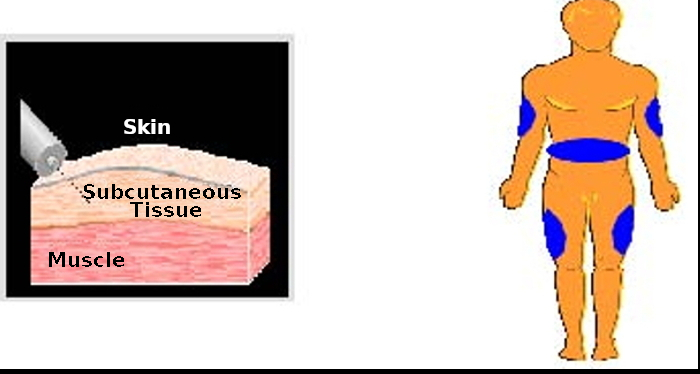
\includegraphics[scale=1.6]{images/088.jpg}\\
\textbf{\textit{Recommended insulin injection sites}}
\end{figure}

\clearpage

\noindent\textbf{Technique of injection}

\vspace{-\topsep}
\begin{enumerate}[•]
\itemsep=0pt
\item Grasp (or gently pinch) a fold of skin at any of the above reco\-mmended body sites.
\item Insert the needle at the bottom of the skin fold at an angle of 90\break degrees or 45 degrees (in thin individuals).
\item Inject insulin and hold needle in position for about 5 seconds to\break ensure all the insulin gets injected.
\item Inject into a different spot each time, but rotate the injection spot within the same area (like the abdominal wall area only, the right thigh only) since this will decrease variability in the amount of drug that enters the blood stream with each injection.
\end{enumerate}


\noindent\textbf{Factors that influence insulin absorption and action}

There is variability in the amount of insulin that enters the blood depending on several factors listed below:

\vspace{-\topsep}
\begin{enumerate}[•]
\itemsep=0pt
\item Potency of the insulin: After opening a bottle of insulin, over time its potency or strength gradually wanes or decreases. In fact it is not recommended to use a bottle 30 days after opening it.
\item Amount of blood flow to the skin site where insulin is injected: For example people who are chronic smokers have reduced blood flow to the skin, and in them, less insulin gets absorbed. On the other hand, after exercise, a hot shower, sitting in a sauna, etc, the blood flow to the skin increases, and this will cause rapid absorption of insulin. Therefore it is recommended to cool off after any of these activities before injecting insulin.
\item The site of injection of insulin: In general insulin injected into the\break abdomen gets absorbed faster than insulin injected into the buttock or thigh. Hence it is recommended to inject rapid– or short–acting insulin into the abdomen, and the slower–acting insulins into\break buttocks and thighs.
\end{enumerate}

\clearpage

\noindent\textbf{Factors that affect your daily insulin requirement}

Over time, most patients figure out how much daily insulin they need to maintain good blood sugar control. This requirement may increase or decrease in the following situations, and hence patients should consult their physician about making slight adjustments in daily insulin intake during these periods.

\vspace{-\topsep}
\begin{enumerate}[•]
\itemsep=0pt
\item Travel: We are likely to eat different kinds of foods (more processed foods in airports, railway stations, bus stations, etc), have more\break irregular eating times (especially during long journeys), and eat\break larger or smaller quantity meals.
\item Eating out: In general when we eat out, we consume a higher amount of calories.
\item Infections: Any kind of infection is likely to increase insulin requirement since the body releases more sugar into the blood during\break periods of stress.
\item Emotional stress: Anger, anxiety, fear and other negative emotions cause our body to release more sugar into our blood.
\item Surgery: Surgery can cause high blood sugar (due to increased\break physical and emotional stress of surgery), or low sugar (due to\break having to be without any food intake before surgeries, or not being able to eat after surgeries).
\end{enumerate}
\vspace{-\topsep}

\noindent\textbf{Storing insulin}

It is important to preserve insulin to maintain its effectiveness.\break Extreme temperature can render insulin impotent. The following\break recommendations should be followed while storing insulin:

\vspace{-\topsep}
\begin{enumerate}[•]
\itemsep=0pt
\item Store insulin in the refrigerator. More specifically, store it in the door pockets, and not inside the refrigerator (shown in picture,\break p. 229). This protects insulin from variations in temperature when we open the refrigerator.

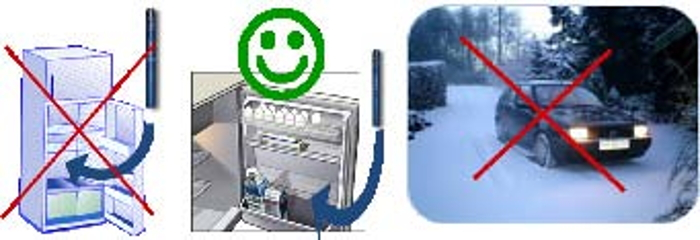
\includegraphics[scale=2.3]{images/089.jpg}

\item Do not store insulin in the freezer.
\item If you experience frequent power outages (power cuts), then\break maintain a cold pack or ice pack to protect insulin.
\item Do not store insulin in the car.
\item Do not store insulin in direct sunlight.
\end{enumerate}
\vspace{-\topsep}

\noindent\textbf{Future trends with insulin}

In future we may expect to see a more convenient form of insulin such as inhaled insulin, oral insulin or insulin patches we can wear. We also expect to see ultra–long acting insulins which you may not have to use daily, but instead once in a few days. In fact, the recently launched ultra–long acting insulin degludec (brand name Tresiba), manufactu\-red by Novo Nordisk, has been approved for use in Europe. Although it is claimed that it can be administered 3 times a week instead of daily injections. It needs to be given daily. It is becoming popular in India.

\noindent\textbf{A final word about the role of medications in diabetes}

Drugs are never a substitute for healthy eating and exercise in the management of type 2 diabetes. While it is convenient to ignore diet and exercise under the false hope that medication(s) or insulin alone will do the job, you are basically fooling yourself and putting your body at risk for complications. All the three components of the triad of\break diabetes management must go hand–in–hand.

\newpage

\chapter{Stress and Diabetes – The Role of Yoga and Meditation (Dhyaana) in Diabetes}\label{chap27}

Stress is a part of everyday life, and has been so from time immemorial. Stress is the body’s response to a threat or adversity, which could\break be real (such as injury or illness) or imaginary (fear, anxiety about something, etc). Stress is an attempt by the body to deal with the\break adversity by what is known as the “flight–or–fight” response, i.e. you will either avoid the problem, or stand up and face it. As part of this process, the body produces several stress hormones. Chief among\break them are adrenaline\index{Adrenaline}, cortisol\index{Cortisol}, glucagon\index{Glucagon} and growth hormone. All these hormones cause more glucose to enter the blood stream because there is an increase in the energy requirement of the human cells as the body deals with the stress. In general, once the source of the stress is gone, the body also relaxes from its hyper vigilant state.

There are two kinds of stress—physical and mental. Physical stress\break includes things such as an injury, illness, surgery, etc. In this chapter we shall focus on mental stress, since this is more prevalent in\break today’s society. So far in the book we have emphasized the management of diabetes at the physical body level, and have illustrated how diet, exercise and medications can help you defeat diabetes and get your life back. We have also acknowledged the contributions of the Western scientists who have worked extensively on this triad of diabetes management. Now it is time to recognize the contributions of Eastern philosophies, and specifically Indian philosophy in preventing and managing a chronic disease state such as diabetes.

\noindent\textbf{How does stress affect diabetes?}

Stress induced neurohormonal excitement results in hypergly\-ce\-mia. If this continues relentlessly, it causes a severe strain on the\break pancreas to constantly produce excess insulin. This will eventually\break result in diabetes in genetically predisposed individuals.

On the other hand, among people who are already diabetic,\break constant or repeated stress will keep the blood sugar levels high and hinder diabetes control. The problem in diabetics is insulin deficiency and insulin resistance, which do not allow the extra sugar that is mobilized by neurohormonal stimulation to enter the cells to provide them more energy needed during periods of stress. Therefore, not only do the cells not get the extra energy they need to function well during stress, there is also an excess amount of unused sugar in the blood. This will increase the risk of long–term complications.

Finally, when individuals are under stress, they may forget to take their medications or insulin, may drink more alcohol, and some people may lose their appetite, while others overeat. All these behaviors will have a negative impact on blood sugar control.

Therefore, stress management is essential to ensure a complica\-tion–free life for diabetics and to prevent diabetes in those indivi\-duals who are at risk for diabetes (pre–diabeties, etc). But herein lies the challenge. In dealing with mental stress we are dealing with an invisible enemy. Your physician can help you cope with the physical stress of dealing with an infection, injury, surgery or other illness, by\break prescribing more insulin, treating the infection or injury, etc. But it is not easy to identify mental stress as the cause of poor diabetes\break control, since most patients do not like to admit they are under stress. Therefore, the best person to help you deal with stress is yourself! You should learn to observe your mood and behavior during different times of the day. Identify daily events that frustrate you. Try to avoid\break situations that cause mental stress. But of course this is easier said than done in today’s world.

Stress is a response or reaction. Instead of attempting to avoid\break adversity (or at least what we perceive as adversity), we are more\break likely to be successful in modifying our attitudes and responses to the various events of daily life. For this, we have to turn to our ancient practices of \textit{yoga} and \textit{dhyaana}. While we have to thank the Western countries for the many innovations and discoveries in the field of\break diabetes, we should be equally proud of our country’s philosophies that have mastered the art of dealing with mental stress.

\noindent\textbf{Stress in the modern day world and the role of the human mind}

Most of the stress we experience in today’s day and age arises\break in the mind. All thoughts, ideas and emotions arise in our mind.\break While positive thoughts, emotions and ideas create a sense of\break well–being and neuro–hormonal balance in the body; negative\break thoughts and emotions create stress and lead to neuro–hormonal\break imbalance and eventually to disease states. Thoughts, emotions and ideas are often a reaction in the mind to an external stimulus. The mind may react negatively to the mundane daily routine such as\break the alarm going off in the morning, navigating the office–hour\break traffic, dealing with your boss or co–workers, or dealing with your\break family. As a result, our nervous system and hormones are always on the edge, never getting a chance to cool off. The consequences of\break this non–stop stress is the explosion in the rates of psychosomatic\break problems such as depression, anxiety, divorce, alcoholism, anger\break issues, high blood pressure, heart disease, and of course diabetes.

The meaning of the word “mind” according to the Oxford Dictionary is “the element of a person that enables them to be aware of the world and their experiences, to think, and to feel; the faculty of consciousness and thought”. While the nervous system controls all bodily\break function through neurotransmitters or chemicals, this nervous\break system is under the control of the mind, and is connected to the mind. The mind decides how we respond to different external stimuli. For\break example, the eyes may see rich or fatty food, and the brain may\break identify the type of food, but it is up to our mind or consciousness to\break decide whether we want to eat this food or not. If the mind\break decides that this food is harmful for our overall well being, then we are not tempted to eat this food. If however, the mind is not disciplined enough, then we succumb to these excesses in life, and these behaviors lay the groundwork for future disease. The mind can also interpret something we read, listen to, or think about in a negative way to create anxiety, anger, depression, frustration, or various other emotions. When a person is in the grip of such negative emotions, he or she is more susceptible to indulge in unhealthy behaviors such as overeating or not eating at all, not being able to sleep or sleeping too much, not having the motivation to exercise and be physically active, not wanting to take essential life saving medications, etc. But the mind also has the power to interpret the same thing in a positive way to create a sense of happiness, pleasure, contentment, and peace. These kinds of emotions are well known to result in positive outcomes. These kinds of people are more likely to eat and sleep properly, be physically active, and indulge in productive activities in the society.

The human mind is so powerful that it does not need an external stimulus to create a thought process. All of us have woken up from a nightmare, sweating, breathing hard and scared. This is purely the work of the imaginative function of the mind! This imaginary world created by the mind seems so real, that our poor body is fooled into thinking it is the truth, and it produces various hormones such as\break cortisol and adrenaline that cause our heart rate, respiratory rate and blood pressure to shoot up!

Thus, the human mind, even though not visible, makes its\break presence felt at every moment. It is obvious that having the right state of mind, will lead us to interpret our surroundings in a positive way, and this leads to making positive choices, and results in positive health outcomes. Mind is the charioteer that steers the five horses, which are our senses, and the chariot, which is our body. If the chario\-teer is weak, then the horses will run helter–skelter. This is the gist of the \textit{Ishopanishath} written by Yajnavalkya, which is widely regarded as the best Upanishad. It emphasizes “\textit{sthithaprajnattva}”, wherein the mind stays stable without reacting to thoughts, emotions or external\break stimuli. A person in this state of mind will automatically be free of disease–causing behaviors, and hence will be free of disease. So how can we control our mind so that it can lead us in the right direction? This fundamental question lies at the heart of our Indian philosophy. Yoga, meditation and prayer are the greatest contributions to the\break world.

Merlene T. Shermann writes in her book “Wellness at the Workplace”, “Cure people’s ills and you can make them happy for a day. Teach them to stay well and you can make them happy and healthy for a lifetime”. The \textit{“sapthapadi”} or seven steps of holistic medicine concept of Indian philosophy aims to do exactly this. It includes diet, supplements, exercise, positive mental attitude, healthy sleep routine, absence of addictions, and the right weight. If we follow this, even if we have a genetic predisposition to develop disease (or diabetes), we can still avoid disease and stay healthy. This was also emphasized by Dr. M. Viswanathan, who was the pioneer of diabetes in India, when he said, “the gun may be loaded, but environment pulls the trigger”.

\vskip 8pt

\noindent{\large\textbf{Role of \textit{Yogaasanas} and \textit{dhyaana} in diabetes}}

\vskip 6pt

\noindent\textbf{What is yoga?}

Yoga means the union of the individual mind with the universal or divine. Yoga is one of the six systems of classical Indian philo\-sophy. The path is described in terms of eight ‘limbs’ called \textit{Yama, Niyama, Aasana, Praanaayaama, Pratyaahaara, Dhaarana, Dhyaana} and \textit{Samaadhi}. But all the eight limbs are beyond the scope of this book; hence only \textit{praanaayaama} and \textit{dhyaana} are described here.

\noindent\textbf{\textit{Praanaayaama}}

Praanaayaama means breath control. \textit{Pranaa}, the vital force of life, flows from the cosmic energy, into us, through our food, water, and air, and becomes our body’s life force. There are several types of Praanaa\-yaamas such as \textit{anulom vilom, kapaalabhathi, ujjayi, udgit, bhastrika,\break suryabhedana}, etc. Each one of them is effective in energizing our\break body’s life force.

As John Douillard, an eminent ayurvedic physician explains in his book, “Body, Mind and Sport, “while we breathe in through the nose, \textit{praana}, which is carried by oxygen, enters the nasal cavity. The air while in the nose is prepared for exchange in the lungs, but the \textit{praana} is said to travel into the brain along the olfactory nerve”. The first stop for the \textit{praana} is the brain, which, when enlivened and energized by it, can coordinate with any or all parts of the body for its various functions.

When we breathe in through the nose, the air passes by small bones in the nose called turbinates, which swirl it into a refined stream most suitable for oxygen exchange. This does not happen when we breathe through the mouth. Instead, the \textit{prana}, along with the unprepared air, moves directly into the lungs. It travels in and out of the body without going to the brain directly through the nasal passages. With proper nasal breathing, says Dr. Douillard, “the role of \textit{praana} is heightened as it is capable of nourishing the control centres of the brain as well as penetrating the deepest level of the lungs and bloodstream”.

Under stress, people tend to breathe rapidly through the mouth. This type of breathing is associated with fear and anxiety, and\break produces activation of the sympathetic nervous system, causing a rush of adrenaline, which triggers glucose release and worsens diabetes.

\noindent\textbf{Yogic practices in diabetes mellitus}

Yoga is an ancient science. It is the jewel in the crown of Indian culture. The need for yoga has never been greater than in today’s world. Several well–planned studies have scientifically evaluated the beneficial effects of yogic exercises/postures on the human body and metabolism. The following health benefits have been documented\break based on many of these studies:

\vspace{-\topsep}
\begin{enumerate}[•]
\itemsep=0pt
\item Decrease in fasting and post–prandial (after food) blood sugars
\item Decrease in HbA1c level
\item Decrease in requirement of oral anti–diabetes medication and insulin dosage
\item Improvement of the so–called “brittle diabetes” or very hard to\break control diabetes seen in some type 1 diabetics.
\end{enumerate}
\vspace{-\topsep}

In addition to these direct improvements in diabetes, the following indirect improvements have also been seen:

\vspace{-\topsep}
\begin{enumerate}[•]
\itemsep=0pt
\item Increase in lean body mass (or muscle mass)
\item Decrease in body fat
\item Decreased insulin resistance and increased insulin sensitivity due to upregulation of insulin receptors
\item Improvement in the lipid profile decrease in triglycerides and chole\-sterol, and increase in HDL (good) cholesterol
\item Decrease in blood pressure levels
\item Decreased mental stress.
\end{enumerate}
\vspace{-\topsep}

\begin{wrapfigure}{r}{5.9cm}
\vskip -.3cm
\centering
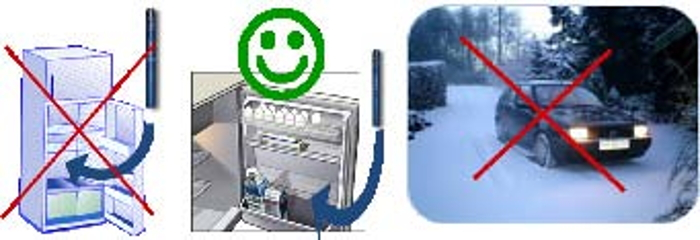
\includegraphics[scale=1.3]{images/090.jpg}\\
\textbf{\textit{Praanaayaama}}
\vskip -.4cm
\end{wrapfigure}

These indirect improvements seen with yoga have the potential to prevent type 2 dia\-betes, or in other words, turn the clock back!

Another interesting observation is that unlike other forms of exercise, yoga increased exercise tolerance\break without increasing oxygen\break consumption and lactic acid formation in the body. Other forms of exercise such as running,\break jogging, etc, cause the oxygen requirement of the muscles to increase. After a period of time, when the body is unable to provide this\break increased oxygen demand, lactic acid begins to accumulate in the\break muscles, which is one of the reasons for us to experience fatigue. But this is not seen with yoga!

The following tables detail the positive outcomes observed among diabetics in experiments conducted at the Vemana Yoga Research Insti\-tute at Secunderabad, India. Dr. Sahay has reported these results in the Journal of Association of Physicians of India (JAPI) in 2007.

{
\begin{table}[H]
\centering
\caption*{\textbf{Effect of \textit{Praanaayaama} on blood glucose}}
\small\addtolength{\tabcolsep}{-4pt}
\begin{tabular}{|l|l|l|l|}
\hline
\multicolumn{1}{|c|}{\multirow{2}{3.2cm}{\textbf{Description of Study}}} & \multicolumn{1}{c|}{\textbf{Type of}} & \multicolumn{1}{c|}{\multirow{2}{.9cm}{\textbf{Before}}} & \multicolumn{1}{c|}{\multirow{2}{.8cm}{\textbf{After}}}\\
 & \multicolumn{1}{c|}{\textbf{Sample}} &  & \\
\hline
Normal volunteers (n=50) & Fasting & 69.05 & 55.23*\\
Immediate effect (1 hr) &  &  & \\
\hline
Type 2 diabetes (n=26); & Fasting & 146.10 ± 43.13 & 106.19 ± 21.05\\
After 1 month & Post prandial & 276.50 ± 43.13 & 166.50 ± 79.37\\
\hline
Type 1 diabetes (n=5); & Fasting & 254.75 ± 179.13 & 126.25 ± 68.02\\
After 1 month & Post prandial & 414.50 ± 175.78 & 275.00 ± 81.34\\
\hline
\multicolumn{4}{@{}l}{*p\textless 0.01}
\end{tabular}
\end{table}
}\relax

{
\begin{table}[H]
\centering
\caption*{\textbf{Glucose and Insulin Levels with Praanaayaama in Type 2 diabetes}}
\small\addtolength{\tabcolsep}{-1pt}
\begin{tabular}{|l|l|l|l|l|l|l|}
\hline
 &  & \multicolumn{1}{|c|}{\textbf{0 hr}} & \multicolumn{1}{c|}{\textbf{½ hr}} & \multicolumn{1}{c|}{\textbf{1 hr}} & \multicolumn{1}{c|}{\textbf{1½ hr}} & \multicolumn{1}{c|}{\textbf{2 hr}}\\
\hline
\multirow{4}{1.5cm}{OGTT\newline (75 gm)\newline (mg/dl)} & Before & 120.0 ± & 222.4 ± & 241.8 ± & 251.8 ± & 242.0 ±\\
 &  & 35.7 & 65.59 & 68.78 & 91.84 & 100.71\\
\cline{2-7}
 & After & 112.2 ± & 192.0 ± & 217.6 ± & 199.8 ± & 197.6 ±\\
 &  & 41.27 & 53.72* & 53.26* & 83.31** & 95.2**\\
\hline
\multirow{4}{1cm}{Insulin/\newline (Glucose)\newline Ratio} & Before & 0.68 ± & 0.16 ± & 0.25 ± & 0.34 ± & 0.18 ±\\
 &  & 0.3 & 0.07 & 0.13 & 0.3 & 0.15\\
\cline{2-7}
 & After & 0.22 ± & 0.24 ± & 0.28 ± & 0.20 ± & 0.30 ±\\
 &  & 0.77 & 0.15 & 0.13 & 0.13 & 0.23*\\
\hline
\multicolumn{7}{@{}l}{*p\textless 0.01, **p\textless 0.001}
\end{tabular}
\end{table}
}\relax

{
\begin{table}[H]
\centering
\caption*{\textbf{Effect of Yoga on the HbA1C and the Drug Score (n=108)}}
\small\addtolength{\tabcolsep}{-2pt}
\begin{tabular}{|l|c|c|}
\hline
 & \textbf{Before} & \textbf{After 3 Months}\\
\hline
Glycosylated Hemoglobin & 10.41 & 8.45*\\
\hline
Drug score & 1.71 & 1.08**\\
\hline
\end{tabular}
\end{table}
}\relax

\clearpage

{
\begin{center}
\small\addtolength{\tabcolsep}{-1pt}
\begin{longtable}{|l|l|l|l|l|}
\multicolumn{5}{@{}c}{{\large\textbf{Blood Glucose values Before / After Different Asanas}}}\\
\hline
\textbf{Groups of} & \multicolumn{2}{c|}{\textbf{Fasting}} & \multicolumn{2}{c|}{\textbf{Postprandial}}\\
\cline{2-5}
\textbf{Asanas} & \multicolumn{1}{|c|}{\textbf{Before}} & \multicolumn{1}{c|}{\textbf{After}} & \multicolumn{1}{c|}{\textbf{Before}} & \multicolumn{1}{c|}{\textbf{After}}\\
\hline
\textbf{Group A} &  &  &  & \\
\hline
\textit{Naavaasana} & 116.8 ± 13.8 & 98.8 ± 9.3* & 223.6 ± 14.6 & 164.6 ± 15.3*\\
\textit{Bhujangaasana} &  &  &  & \\
\hline
\textbf{Group B} &  &  &  & \\
\hline
\textit{Halaasana} & 135.6 + 21.6 & 121.6 + 15.7 & 271.9 + 36.3 & 187.8 + 38.0**\\
\textit{Vajraasana} &  &  &  & \\
 \hline
\textbf{Group C} &  &  &  & \\
\hline
\textit{Yogamudra} & 94.6 + 14.8 & 108.2 + 10.9 & 217.8 + 24.8 & 189.1 + 16.7\\
\textit{Shalabhaasana} &  &  &  & \\
 \hline
\textbf{Group D} &  &  &  & \\
\hline
\textit{Dhanuraasana} & 168.7 + 19.3 & 120.8 + 9.2 & 322.0 + 40.3 & 194.0 + 19.6*\\
\textit{Ardhamatsye-} &  &  &  & \\
\textit{ndraasana} &  &  &  & \\
\hline
\end{longtable}
\end{center}
}\relax


\vspace{-\topsep}
\begin{figure}[h]
\vskip -.5cm
\centering

\includegraphics[scale=1.6]{images/091.jpg}\\
\textbf{\textit{Bhujangaasana}}
\vskip -.5cm
\end{figure}

\begin{center}
\begin{tabular}{@{}cc@{}}
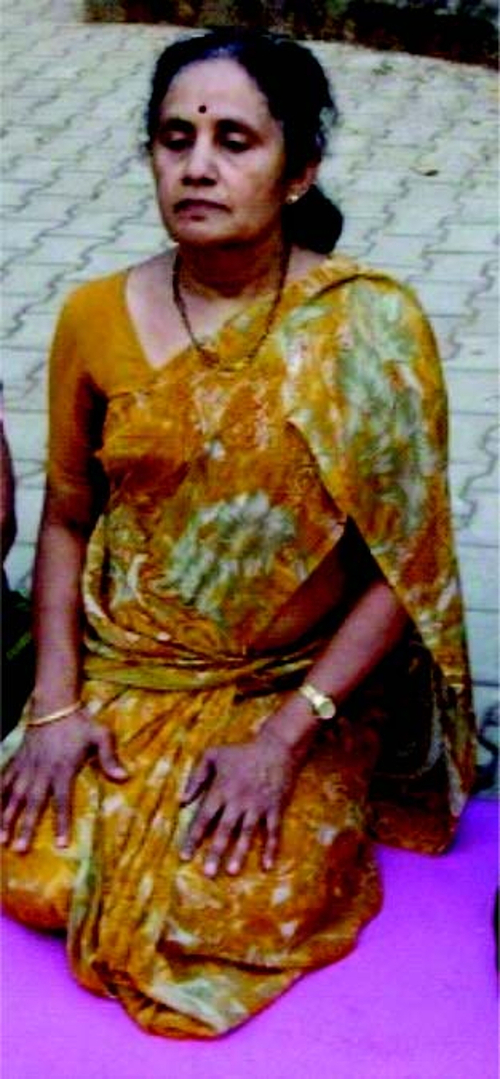
\includegraphics[scale=.6]{images/092.jpg} &
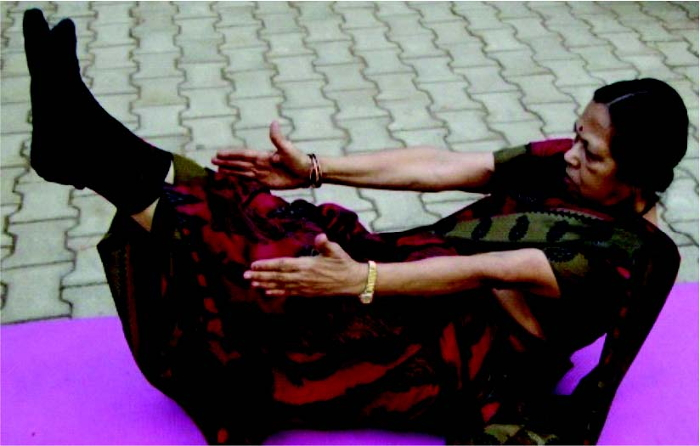
\includegraphics[scale=1]{images/093.jpg}\\
{\textbf{\textit{Vajraasana}}} &
{\textbf{\textit{Naavaasana}}}\\
\end{tabular}
\end{center}

\clearpage

\begin{figure}[h]
\centering
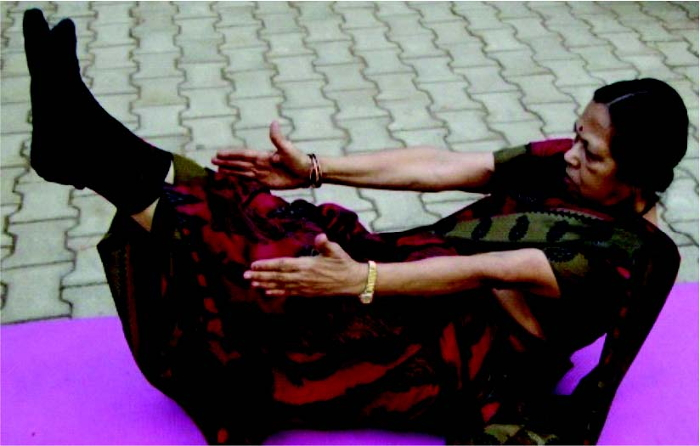
\includegraphics[scale=1.8]{images/094.jpg}\\
\textbf{\textit{Shavaasana}}
\end{figure}


\noindent{\large\textbf{\textit{Dhyaana} In diabetes}}

\begin{wrapfigure}{r}{5cm}
\vskip -.4cm
\centering
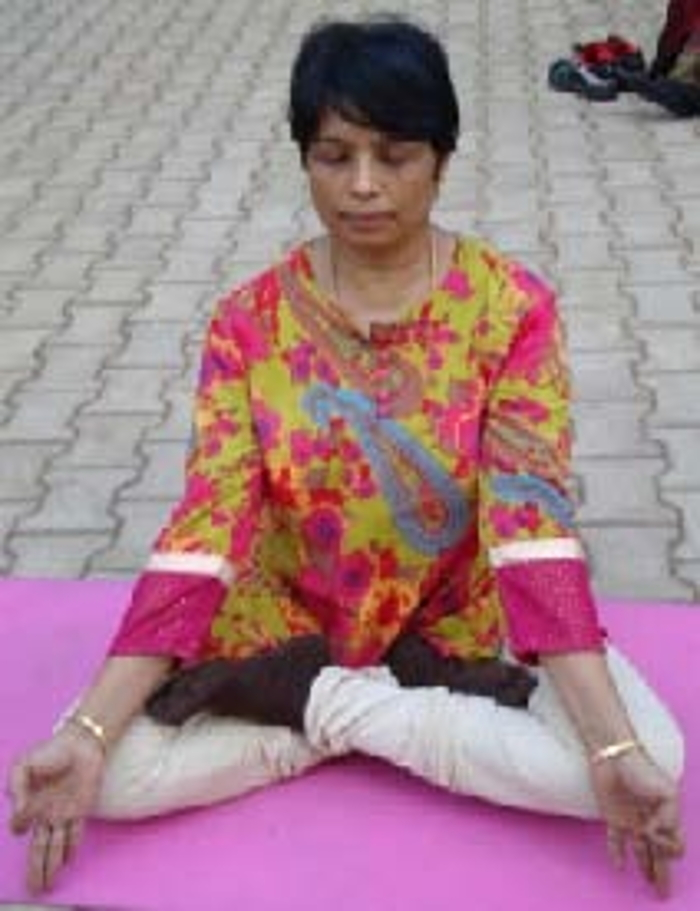
\includegraphics[scale=1.1]{images/095.jpg}
\vskip -.4cm
\end{wrapfigure}

\textit{Dhyaana} is the Sanskirt word for meditation. It is a mental exercise\break for the purpose of achieving greater spiritual heights. It is a means of achieving tranquility of the mind. The human mind in its essence is\break tranquil like the depths of a lake. But just as the lake is more turbulent on its surface, the human mind can get agitated as it deals with the mundane daily routines. Thoughts, memories, and negative feelings constantly disconcert the mind. But \textit{dhyaana} is a state of “just being”, without judging, thinking, or reacting. It teaches us to observe our reactions without getting emotionally attached to them. It teaches us to be a “detached witness” to our own state of mind without judging self or other. Gradually as you practice\break meditation, your mind becomes calm and you can transcend surface emotions and reactions, and dive into the tranquility that\break exists in the depths of our being. Life is ordinarily thought to consist of three states of mind– wakeful state, dream state and sleep. But beyond this is a fourth state called \textit{turiya}. \textit{Dhyaana} allows us to reach this state, which is called \textit{sat–chit–aananda}. In this state there is no good or bad, and we are at peace. Practicing dhyaana daily will give us a taste of \textit{sat–chit–aananda}. We can now perform our daily routine in this state of mind, where there is no negativity, and the possibilities are boundless.

The relevance of \textit{dhyaana} in diabetes is that this positive state\break of mind influences the neurons and hormones in the body to create\break more harmony and less stress, and hence less insulin resistance and hyperglycemia.

There are various schools of thought to the practice of \textit{dhyaana} and yoga. The best among them are said to be:

\vspace{-\topsep}
\begin{enumerate}[•]
\itemsep=0pt
\item \textit{Vipassana} technique (described by Mr. S.N. Goenka).
\item \textit{Kriya yoga} (described in “Autobiography of a Yogi” by Paramahamsa Yogananda) yogada satsangh society.
\item \textit{Ashtaanga Yoga} popularized by B.K.S. Iyengar and Pattabhi Jois.

\textit{Dhyaana} should help you transcend the mind. But the human\break mind is very powerful. Let it not fool you into thinking \textit{dhyaana} is an alternative to healthy eating, exercise and medications. \textit{Dhyaana} should not become an excuse for gluttony and laziness. In fact, this would be a grave disservice to this ancient Indian practice. A true yogi who performs \textit{dhyaana} is in tune with the cosmic. Healthy\break eating, staying active, and tranquility of the mind are a way of\break life for these indi\-viduals. There is no place for sloth, gluttony and negativity in such a life.
\end{enumerate}


\chapter{Alcohol, Tobacco Smoking \& Diabetes}\label{chap28}

\vspace{-\topsep}
{\noindent\Large\textbf{1. Alcohol and diabetes}}

Alcohol is probably the oldest drug known to mankind. Just like anything else we consume alcohol, which affects blood sugar. While most people may be aware of the effects of different types of foods on diabetes, very few may be aware of the effect of alcohol on blood sugar. Did you know that drinking alcohol can actually lead to low blood sugar! Let us try to understand how this can happen.

Alcohol is the second fastest absorbed substance into our body,\break the first being water. It enters the blood in less than 5 minutes\break after consumption. It is metabolized by the liver. The liver needs about two hours to metabolize 1 drink (1 ounce or 30 ml of whiskey or any other hard liquor). During these two hours, other biochemical functions of the liver slow down. When people do not eat any food while drinking alcohol, the body has to rely solely on the glucose stores for its energy needs. Glucose is stored as glycogen in the liver. This store gets depleted in 1-2 days without being replenished. Moreover, the conversion of glycogen to glucose in the liver is slower when the liver is also metabolizing alcohol.

Another glucose source for the body during periods of no food\break intake is gluconeogenesis. This is a process when the protein in\break muscles, and fat stores are converted to glucose. This process is also slowed down when the liver is metabolizing alcohol. 

Therefore, when people consume alcohol without eating food, the liver is unable to efficiently utilize storage forms of glucose (glycogen), or efficiently convert protein or fat into glucose (gluconeogenesis), and these factors can lead to low blood sugar levels.

To complicate matters, an intoxicated person could mistake\break symptoms of hypoglycemia and instead attribute them to being drunk. 

When hypoglycemia does result, the body tries to counter this by releasing glucagon, which tries to raise the blood sugar level. But this process is inhibited during alcohol consumption. 

Unchecked, this situation could lead to hypoglycemia coma!

\noindent Other deleterious effects of alcohol include:

\vspace{-\topsep}
\begin{enumerate}[•]
\itemsep=0pt
\item Increase in triglyceride levels
\item Increase in uric acid levels which can cause gout
\item Disruption of healthy eating habits, because people seldom think\break about eating healthy foods when inebriated
\end{enumerate}
\vspace{-\topsep}

Adults with diabetes do not have to abstain from alcohol. Indeed, the guidelines for alcohol use in individuals with diabetes mirror those for the general population. However, restrictions or abstinence from alcohol are necessary in some situations as explained below:

Regardless of the ills of alcohol, it is a hard habit to overcome. But there are ways to reduce the potential harm of alcohol by adopting the following measures:

\vspace{-\topsep}
\begin{enumerate}[•]
\itemsep=0pt
\item Never drink on an empty stomach
\item Drink with a meal or after a meal
\item Drink in moderation
\item Drink slowly (1 drink over an hour)
\item Do not drink if your blood sugar level is not well controlled
\item Do not binge drink
\item Keep a source of glucose with you all the time in case you get hypo\-glycemia
\item Do not drink and exercise, both can cause hypoglycemia
\item Do not drink and drive a vehicle
\end{enumerate}

In addition, the following subset of diabetics should completely avoid alcohol:

\vspace{-\topsep}
\begin{enumerate}[•]
\itemsep=0pt
\item Pregnant women (because alcohol passes through the placenta to reach baby’s blood stream and causes fetal alcohol syndrome)
\item Poorly controlled diabetics
\item Diabetics with neuropathy
\item Diabetics with hypertriglyceridemia
\item Patients with a history of pancreatitis (or inflammation of the pancreas)
\item Obese individuals (because it contributes to obesity)
\end{enumerate}
\vspace{-\topsep}

General recommendations for alcohol use is not more than 2 ounces per day for men and one ounce for women.

\noindent An alcohol measure means:

\vspace{-\topsep}
\begin{enumerate}[•]
\itemsep=0pt
\item 1 ounce of alcohol is 30 ml.
\item 5 ounces of wine is equal to 30 ml liquor.
\item 12 ounces of Beer is equal to 30 ml of liquor
\end{enumerate}
\vspace{-\topsep}

\noindent\textbf{Interaction between Alcohol and Antidiabetic drugs:}

Alcohol along with insulin over dosage can result in hypoglycemia. Although here is a limited information on the interaction between oral drugs like sulphonyureas (eg Glimiperide, glyclazide etc) they can\break cause hypoglycemia. Therefore the dosage shall be adjusted along with alcohol intake as per the guidelines of the family physician.

{\noindent\Large\textbf{2. Tobacco and Diabetes:}}

The history of smoking dates back to 5000 BC in the shamanistic rituals. Using tobacco in any form is injurious to health.

It is surprising to note that smoking is associated with the\break development of diabetes as per the numerous prospective studies. One such study is “Nurses Health study”$^{\text{\cite{chap28–key01}}}$$^,$$^{\text{\cite{chap28–key02}}}$$^,$$^{\text{\cite{chap28–key03}}}$. Another surprise is that smoking is associated with higher bad cholesterol levels and lower good cholesterol levels besides resistance to insulin action.

Tobacco smoking is like a slow poison to the blood vessels of a\break diabetic.

How is it? Let’s know.

Diabetes alone causes twin complications to the blood vessels:

A - Microvascular disease, meaning those damages that are not\break visible to the naked eye but visible through the microscope.

B - Macrovascular disease, meaning they are directly visible to the eye.

Because of twin damages, the diameter of the blood vessels\break gradually gets reduced in such a way the patency is narrowed and blood flow compromised.

When smoking is added to the compromised state of the blood\break vessels, it causes hardening of the inner walls and pasting of the\break cholesterol plaques to the inner walls. The walls of the blood vessels become damaged, stiff and the ability of contraction and relaxation is lost culminating in compromised blood circulation in the feet. When there is an injury to the feet, due to lack of nourishment to that part of the feet, healing of the wound gets delayed and infected, leading to amputation. So, “stop smoking and save feet”.

Smokers are 30-40\% more likely to develop type 2 diabetes than non smokers. The more one smokes the higher the risk of diabetes.  Also, smoking makes diabetes harder to control$^{\text{\cite{chap28–key01}}}$. Diabetics who\break smoke also have an increased risk of serious complications such as:

\vspace{-\topsep}
\begin{enumerate}[•]
\itemsep=0pt
\item Cardiovascular disease and stroke
\item Kidney disease
\item Diabetic foot disease
\item Diabetic retinopathy
\item Diabetic neuropathy
\end{enumerate}
\vspace{-\topsep}

Therefore, simply put, there is no advice other than to quit\break smoking completely.

\vspace{-\topsep}
\begin{thebibliography}{99}
\vspace{-\topsep}
\itemsep=0pt
\bibitem{chap28–key01} Rimm EB, Manson JE, Stampfer MJ, et al.: Cigarette smoking and the risk of diabetes in women. \textit{Am J Public Health} 1993;83(2):\break 211–214.
\bibitem{chap28–key02} Rimm EB, Chan J, Stampfer MJ, et al.; Prospective study of cigarette smoking, alcohol use, and risk of diabetes in men. BMJ 1995;310(6979):555–559.
\bibitem{chap28–key03} Will JC, Galuska DA, Ford ES, et al.: Cigarette smoking and dia\-betes mellitus: Evidence of a positive association from a large\break prospective cohort study. \textit{Int J Epidemiol} 2001;30(3):540–546.
\bibitem{chap28–key04} U.S. Department of Health and Human Services. \textcolor{blue}{The Health\break Consequences of Smoking—50 Years of Progress: A Report of the Surgeon General.} Atlanta: U.S. Department of Health and Human Services, Centers for Disease Control and Prevention, National Center for Chronic Disease Prevention and Health Promotion,\break Office on Smoking and Health, 2014 [accessed 2019 June 23].
\bibitem{chap28–key05} U.S. Department of Health and Human Services. \textcolor{blue}{A Report of\break the Surgeon General. How Tobacco Smoke Causes Disease: What\break It Means to You.} Atlanta: U.S. Department of Health and Human Services, Centers for Disease Control and Prevention, National Center for Chronic Disease Prevention and Health Promotion,\break Office on Smoking and Health, 2010 [accessed 2019 June 23].
\bibitem{chap28–key06} Guidelines for use of alcohol, page 624, 1154 Joslin’s Diabetes\break Mellitus 14$^{\text{th}}$ Edn.
\end{thebibliography}

{\Large
\noindent\textbf{Conclusions:}

\vspace{-\topsep}
\begin{enumerate}[•]
\itemsep=0pt
\item \textbf{Diabetes has reached epidemic proportions\break globally and in India.}
\item \textbf{Any number of doctors, any number of Governments, any number of NGO's will not be able to contain Global Diabetes menace unless preven\-tive steps are taken at all levels starting from adolescence in the population. Creating global awareness on diabetes is the mantra for primary prevention.}
\item \textbf{Many complications due to uncontrolled hyperglycemia, and associated comorbidities.}
\item \textbf{Multiple treatment paradigms and existing\break guidelines.}
\item \textbf{Need of therapy that not only targets glycaemic control but also takes care of associated comorbidities, prevents com\-plications and avoids\break adverse events of medications.}
\item \textbf{Each patient is unique and individualization of treatment is the only key!}
\end{enumerate}

}

